% (C) Marc Lijour, 2019 
% Licensed under a Creative Commons License BY-SA
% https://creativecommons.org/licenses/by-sa/2.5/ca/
% Presentation at the Toronto French Business Network
% Identity and Blockchain
% Presentation touching upon:
% - blockchain 101
% - identity
% - self sovereign identity
% - applications
% 
\frame{
	\frametitle{This panel is brought to you by}
	\begin{columns}[T]
	\column{0.5\textwidth}
	\vspace{1em}
	\begin{figure}
		
\includegraphics[width=4cm]{../../pics/logos/LogoTFBN}
	\end{figure}
	\center\Large
	\vspace{-1em}
	\url{https://www.tfbn.ca}
	\column{0.5\textwidth}
	\vspace{2em}
	\begin{figure}
		
\includegraphics[width=6cm]{../../pics/logos/gowling}
	\end{figure}
	\center\Large
%	\vspace{-2em}
	\url{https://gowlingwlg.com}
	\end{columns}
}

\frame{
	\frametitle{Access these slides online}
	\center\Huge 
	\url{https://bit.ly/2IdhOFl}\\ 
	\vspace{2em}
	{\normalsize 
		or at\\
		\url{https://github.com/marclijour/presentations}
	}
}

% ======================================================================================================
%                         Blockchain 101 
% ======================================================================================================
\section{What is Blockchain?}
\frame{
	\frametitle{The Trust Machine}
	\begin{figure}
		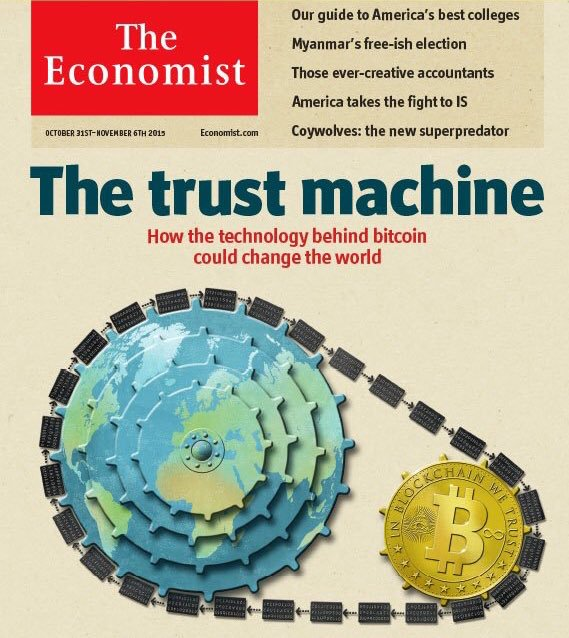
\includegraphics[height=6cm]{../pics/blockchain/economist-trust-machine}
	\end{figure}
}

\frame{
	\frametitle{But how does it work?}
	\begin{figure}
		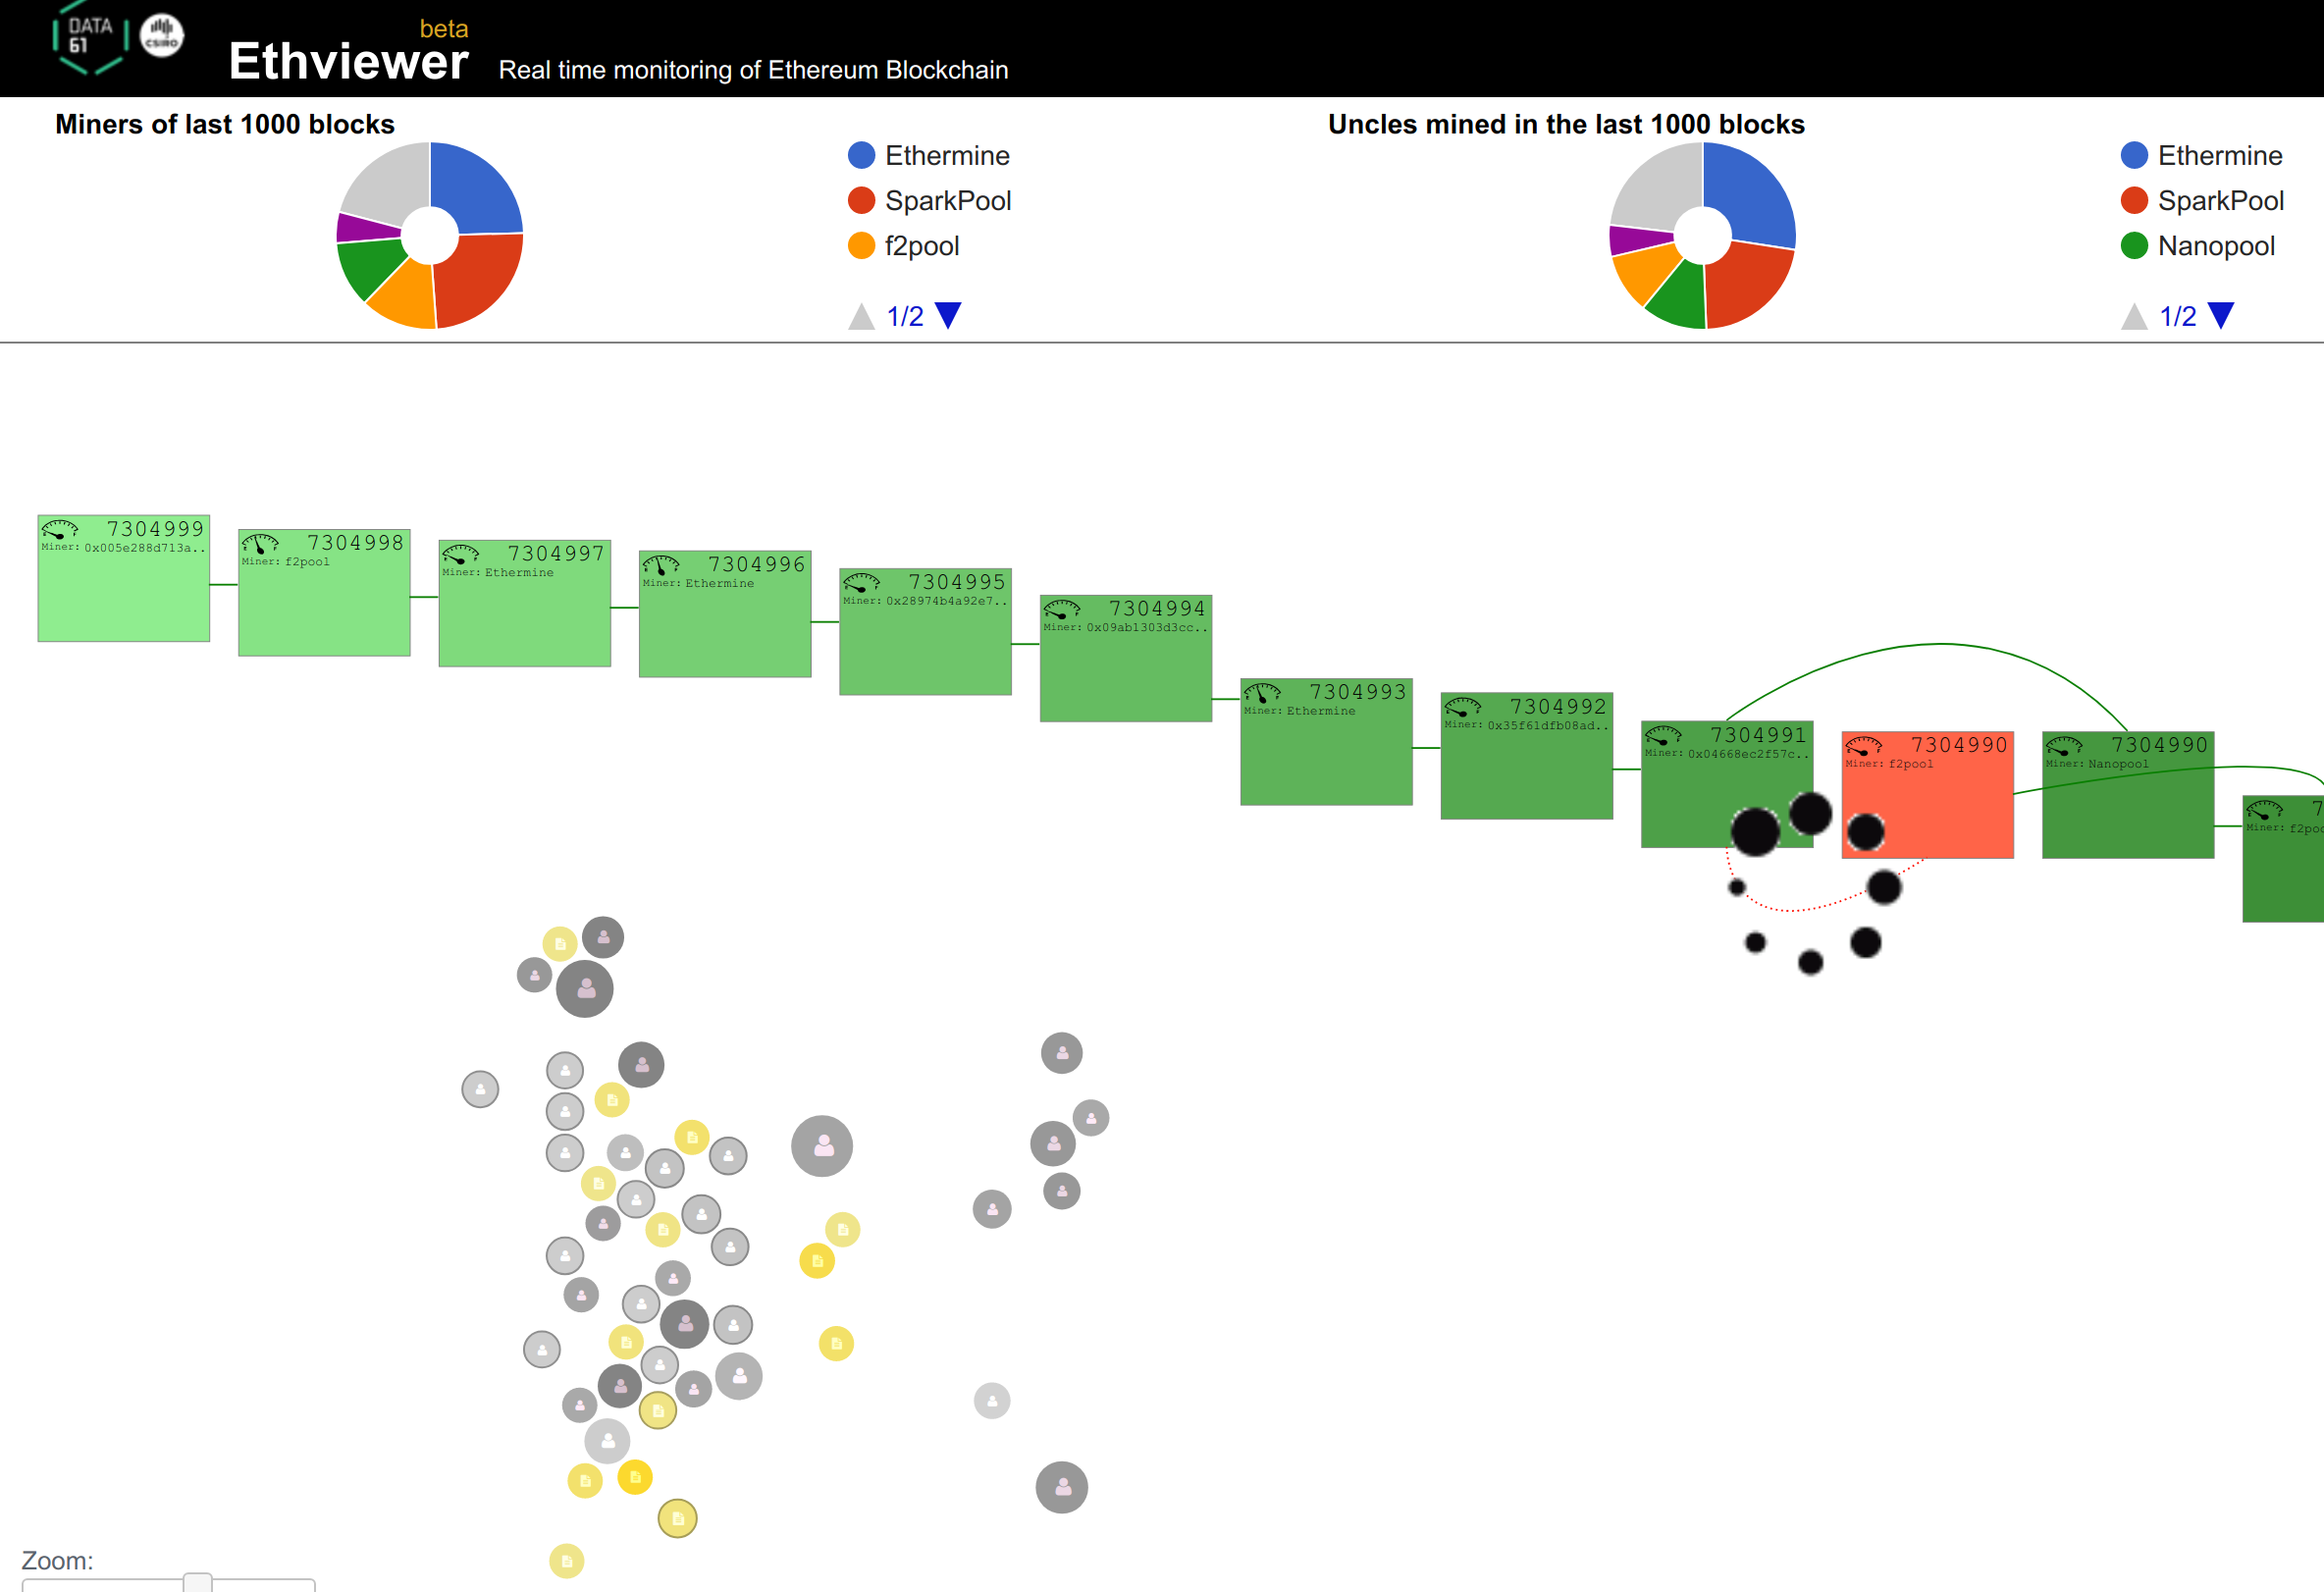
\includegraphics[height=6cm]{../pics/ethereum/ethviewer}
		\captionsetup{justification=centering}
		\caption{Source~: \url{http://ethviewer.live}}
	\end{figure}
}

\frame{
	\frametitle{Reference books}
	\framesubtitle{Blockchain in practice}
	\begin{columns}[T]
	\column{0.5\textwidth}
		\begin{figure}
			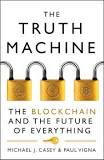
\includegraphics[height=4cm]{../pics/books/book-casey-truth.jpeg}
			\captionsetup{justification=centering}
			\caption{Book from \cite{casey2018:truth}}
		\end{figure}
	\column{0.5\textwidth}
		\begin{figure}
			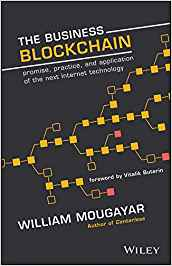
\includegraphics[height=4cm]{../pics/books/book-mougayar-business}
			\captionsetup{justification=centering}
			\caption{Book from \cite{mougayar:business}}
		\end{figure}
	\end{columns}
}

\frame{
	\frametitle{Ultimate references}
	The must-read white paper from legendary Satoshi Nakamoto: \textit{Bitcoin: A Peer-to-Peer Electronic Cash System} (\citeyear{satoshi:bitcoin-paper}),\\
	\vspace{1em}
	the Ethereum white paper from home-town Toronto Vitalik Buterin: \textit{A Next-Generation Smart Contract and Decentralized Application Platform} (\citeyear{buterin:ethereum-paper}),\\
	\vspace{1em}
	and the yellow paper authored by Prof. Gavin Wood: \textit{Ethereum: A secure decentralised generalised transaction ledger} (\citeyear{wood:ethereum-yellow-paper}).
}

% ======================================================================================================
%                         Identity 
% ======================================================================================================
\section{Identity and Blockchain}
\frame{
	\frametitle{Blockchain is not the solution to everything}
	\begin{figure}
		
\includegraphics[height=6cm]{../pics/blockchain/thor-hammer}
	\end{figure}
}

\frame{
	\frametitle{Digital identity}
	\begin{figure}
		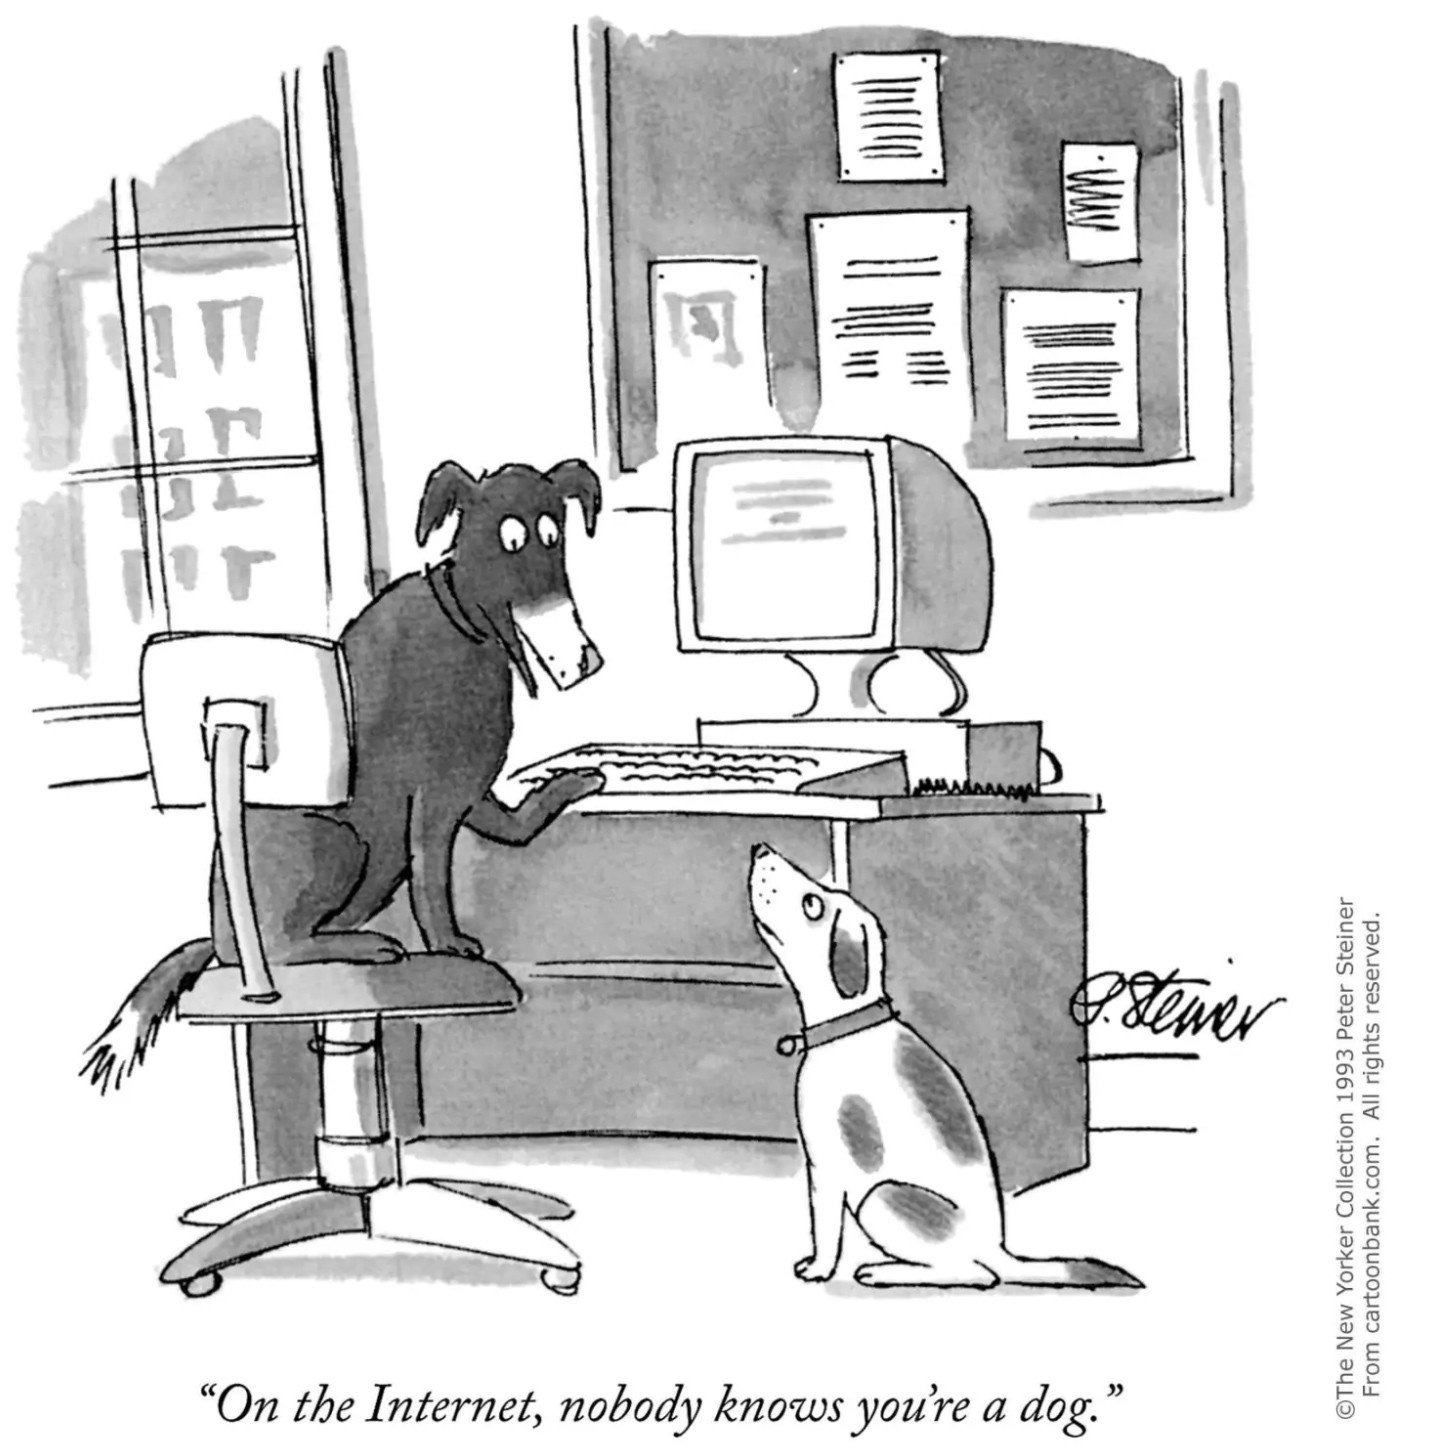
\includegraphics[height=6cm]{../pics/identity/dog-nobody-knows}
	\end{figure}
}

\frame{
	\frametitle{Why is Digital Identity important?}
	\framesubtitle{From Christine Leong (\citeyear{cleong2019:idimportant}), MD and Global Lead for Identity Innovation}
	\begin{figure}
		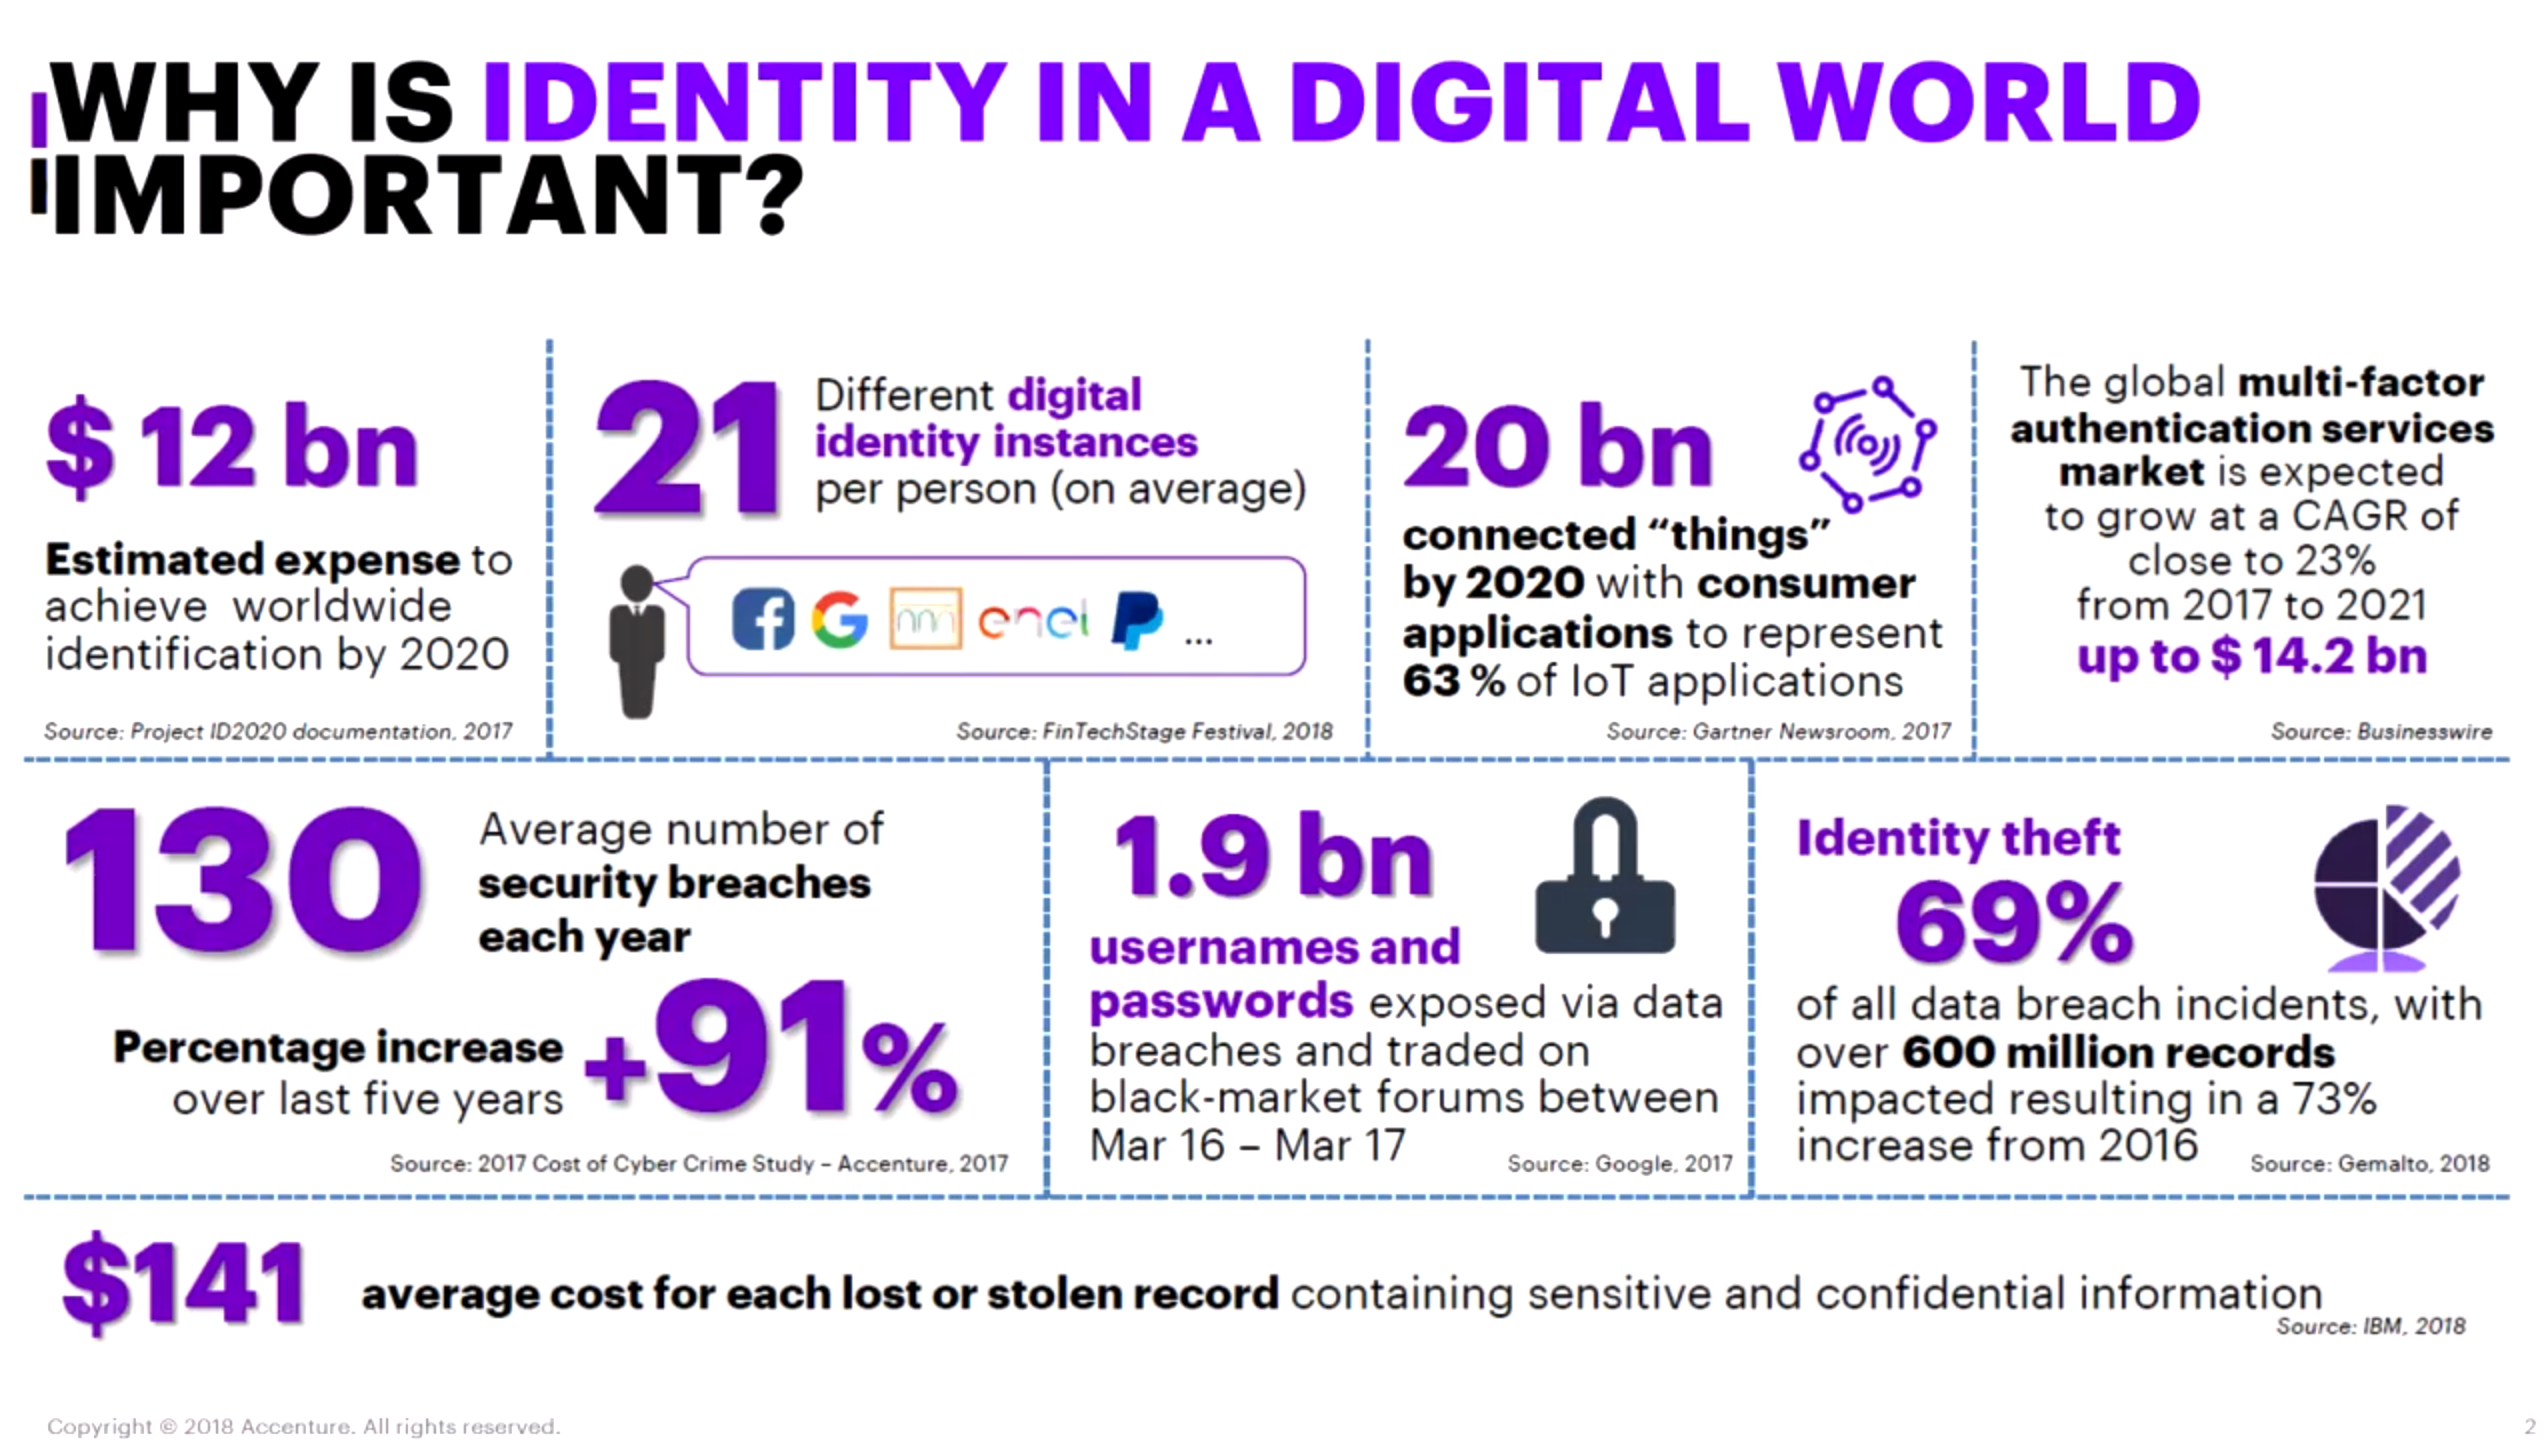
\includegraphics[height=7cm]{../pics/identity/cleong-accenture-2019-id-stats}
	\end{figure}
}

\frame{
	\frametitle{Digital identity Management Paradigms}
	\begin{figure}
		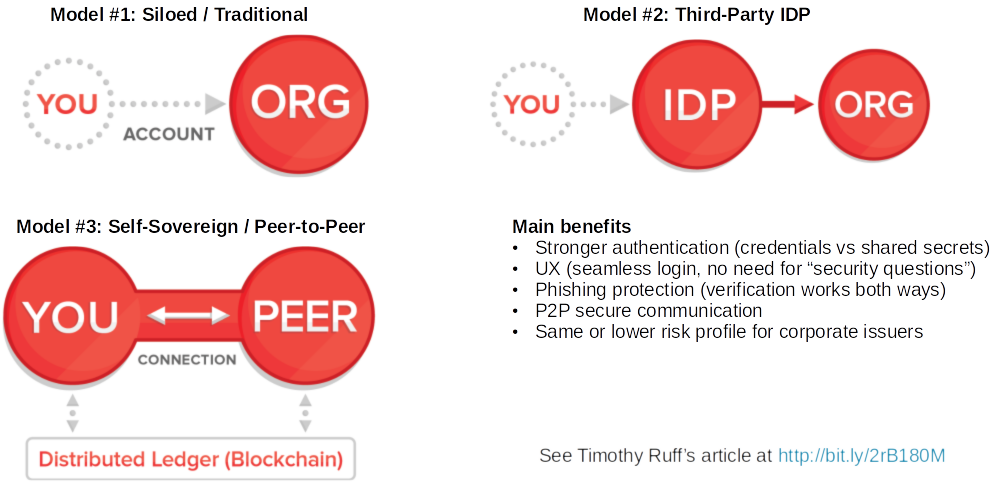
\includegraphics[height=6cm]{../pics/identity/ruff-board}
			\captionsetup{justification=centering}
			\caption{extract from \cite{ruff:id-types}}
	\end{figure}
}

\frame{
	\frametitle{Self-Sovereign Identity in practice}
	\framesubtitle{Extract from the white paper from \cite{sovrin-white-paper}}
	\begin{figure}
		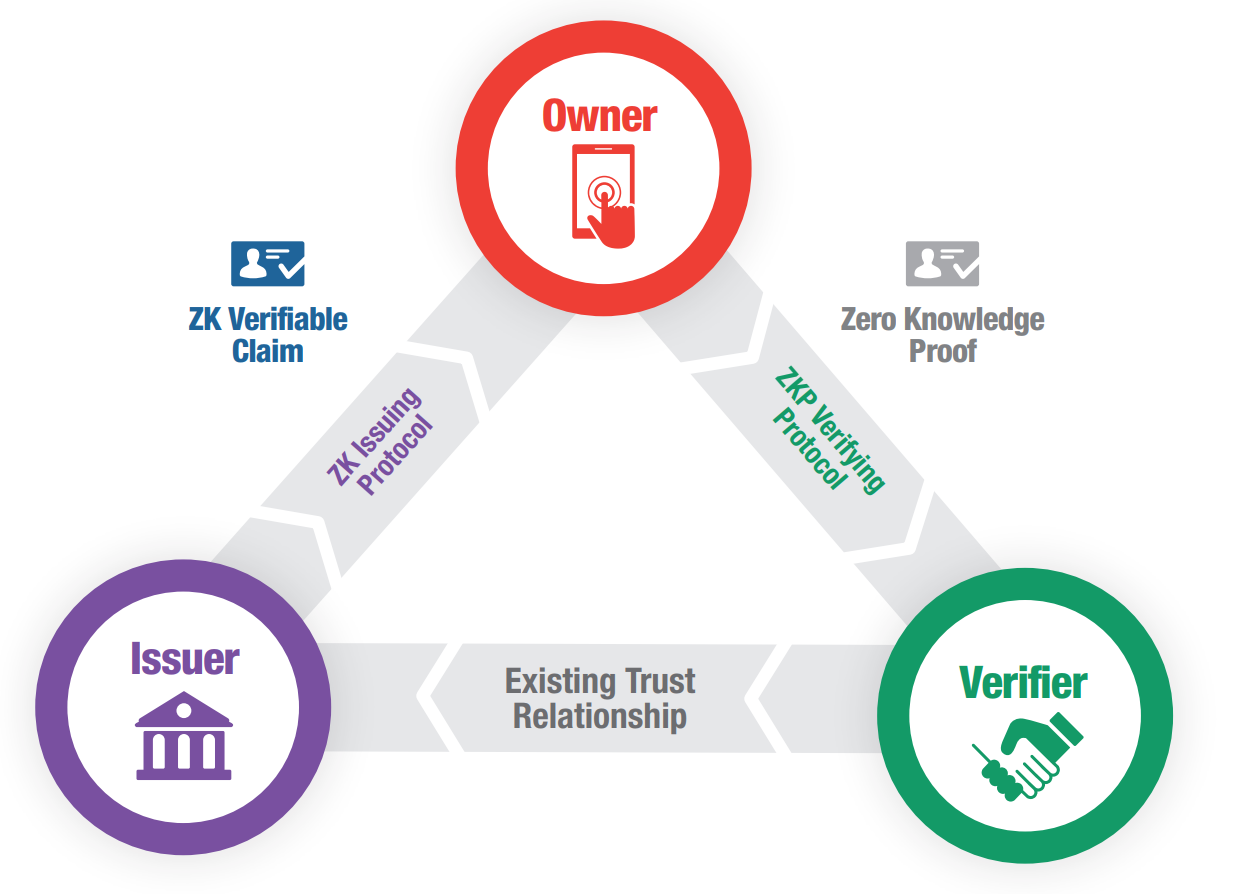
\includegraphics[height=6cm]{../pics/identity/sovrin-zkp}
	\end{figure}
}

\frame{
	\frametitle{The SSI Stack for portable identities}
	\framesubtitle{From \cite{terbu2019:ssi-stack}}
	%\framesubtitle{\url{https://medium.com/decentralized-identity/the-self-sovereign-identity-stack-8a2cc95f2d45}}
	\begin{figure}
		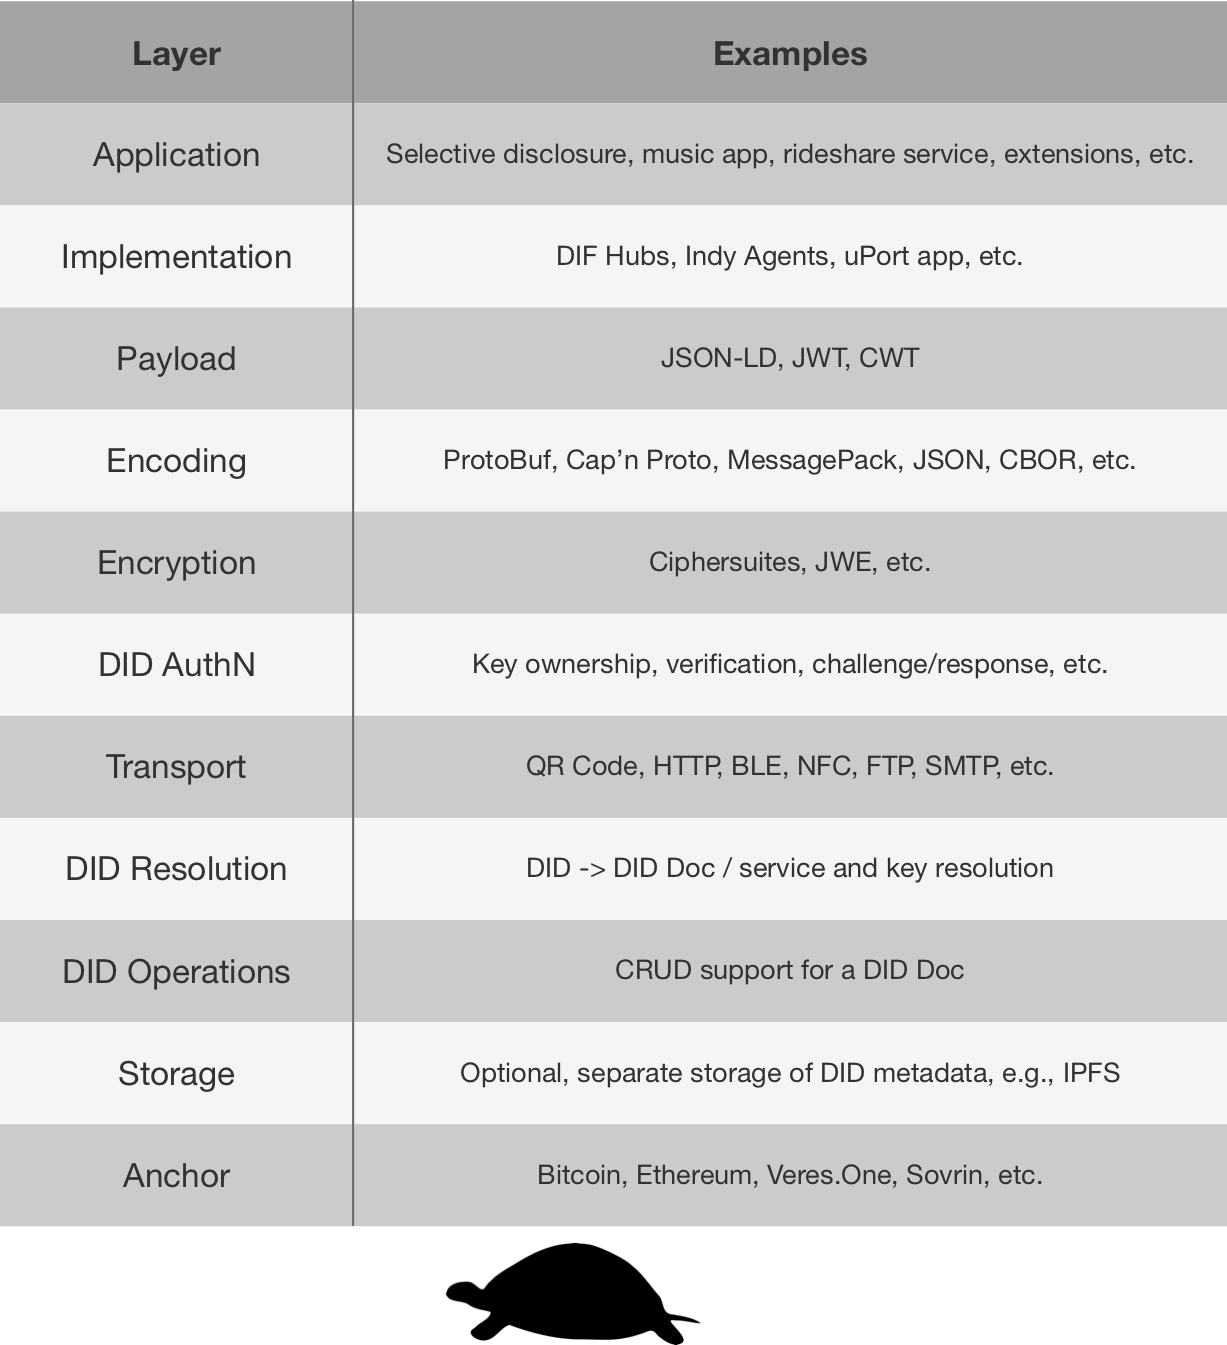
\includegraphics[height=6cm]{../pics/identity/ssi-stack}
			\captionsetup{justification=centering}
			\caption{\textit{based on the results of the workshop (...) provided by Kyle Den Hartog (Evernym) and Daniel Buchner (Microsoft)}}
	\end{figure}
}

\frame{
	\frametitle{Ten Principles of Self-Sovereign Identity}
	\framesubtitle{From \cite{rwot2-id2020-path-to-ssi}}
	\begin{enumerate}
		\item Existence
		\item Control
		\item Access
		\item Transparency
		\item Persistence
		\item Portability
		\item Interoperability
		\item Consent
		\item Minimilization
		\item Protection
	\end{enumerate}
}

\frame{
	\frametitle{The W3C work on DIDs and Verifiable Credentials}
	\framesubtitle{\url{https://w3c-ccg.github.io/did-primer/}}
	\begin{figure}
		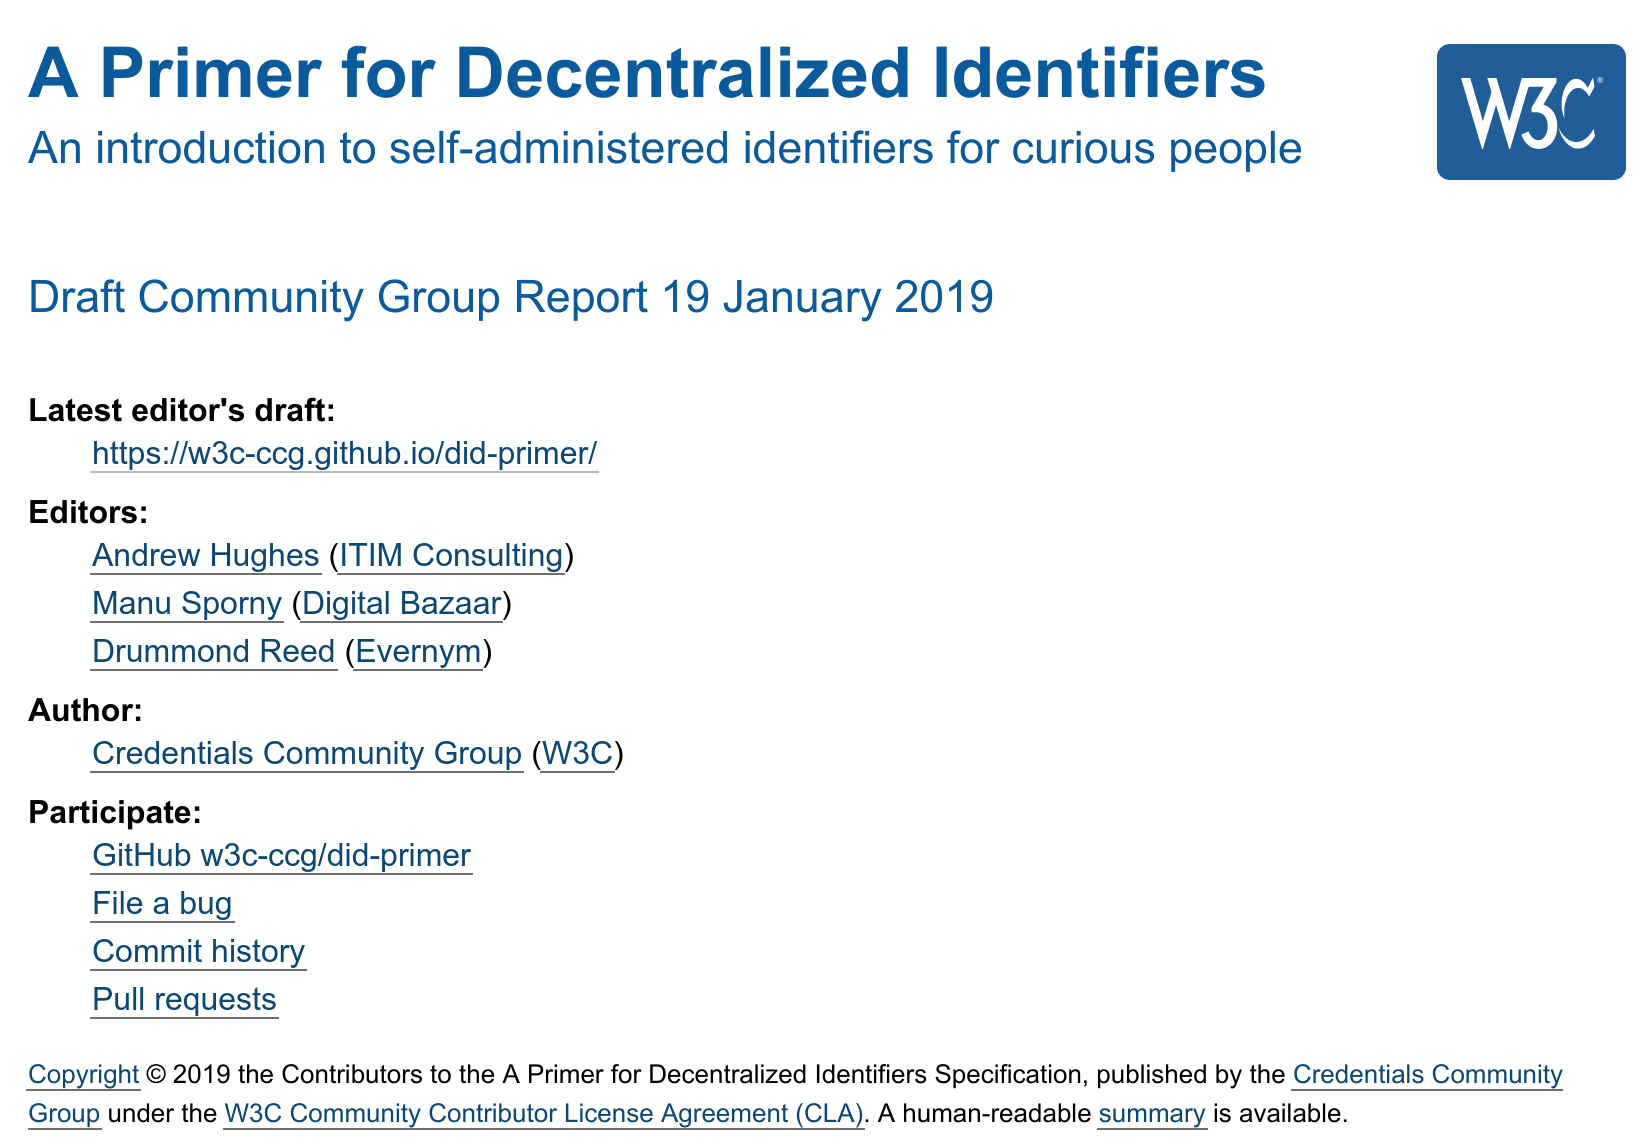
\includegraphics[height=6cm]{../pics/identity/w3c-did-primer}
	\end{figure}
}

\frame{
	\frametitle{Decentralized Identity Foundation}
	\framesubtitle{\url{https://identity.foundation}}
	\begin{figure}
		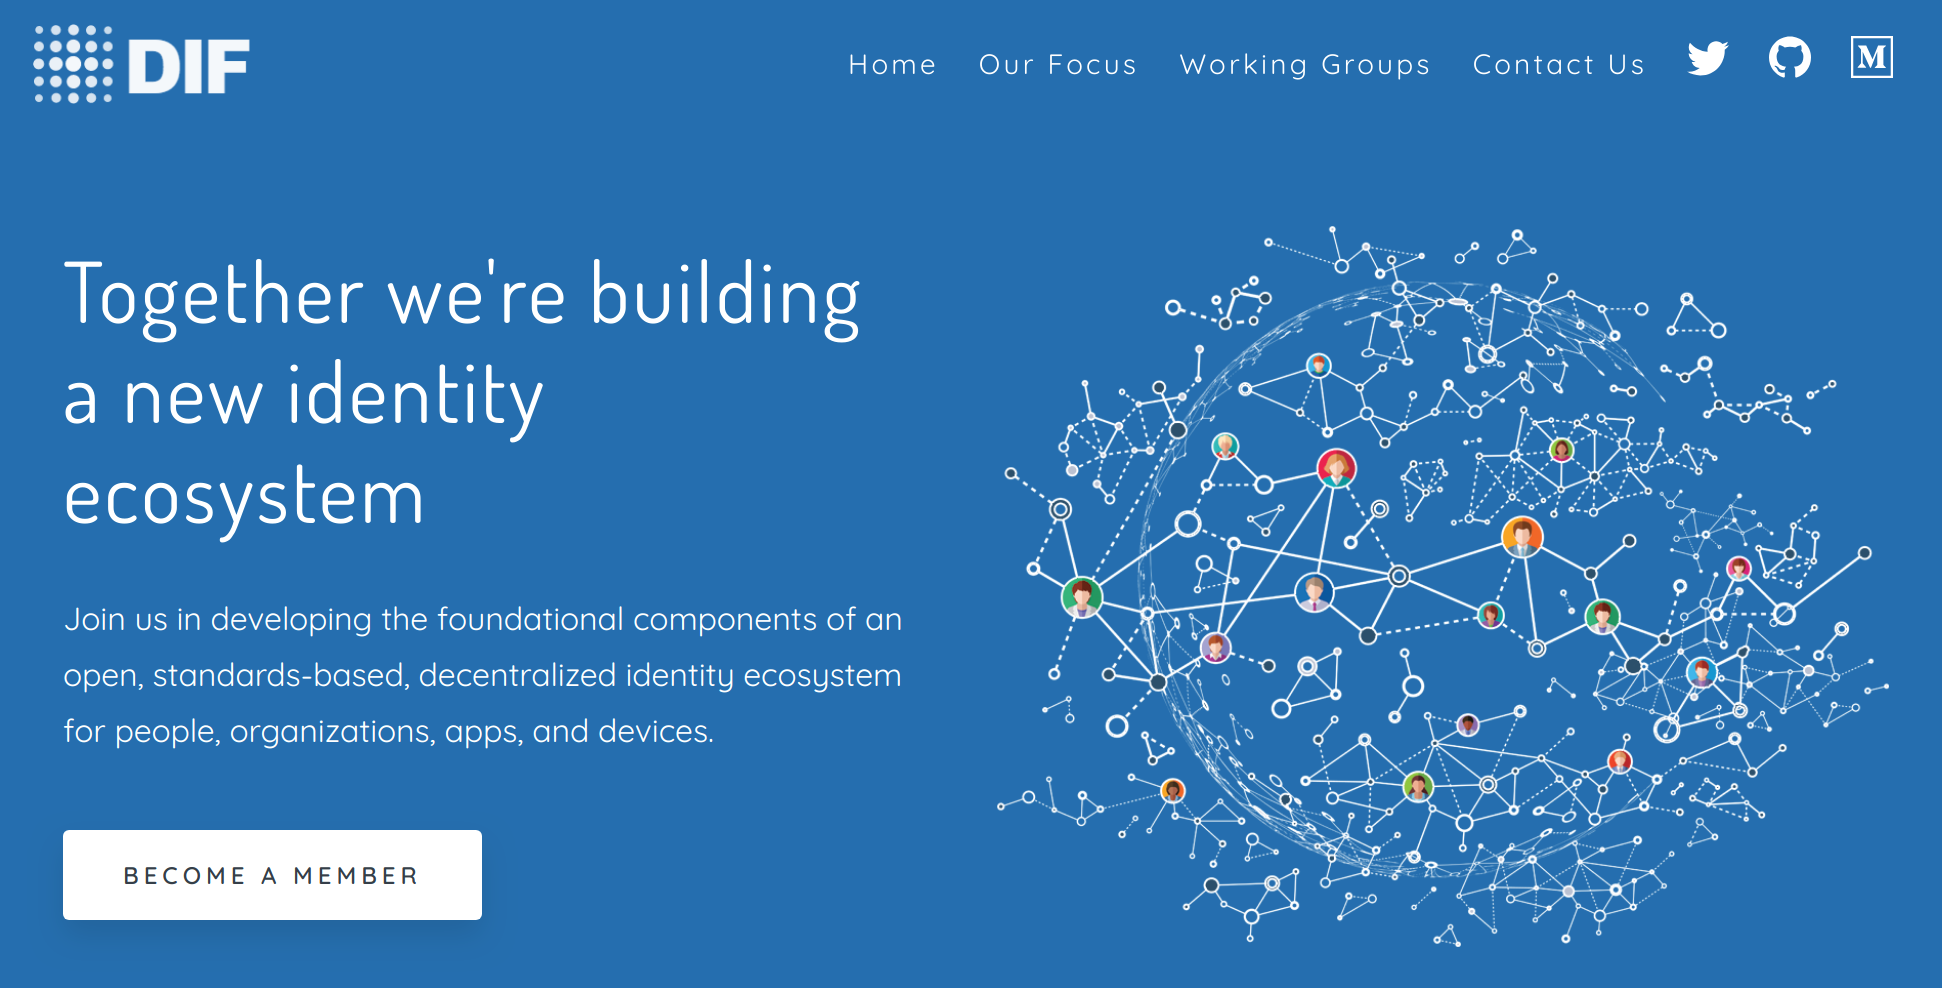
\includegraphics[height=6cm]{../pics/identity/dif}
	\end{figure}
}

\frame{
	\frametitle{Digital Identification and Authentication Council of Canada (DIACC)}
	\framesubtitle{\url{https://diacc.ca}}
	\begin{figure}
		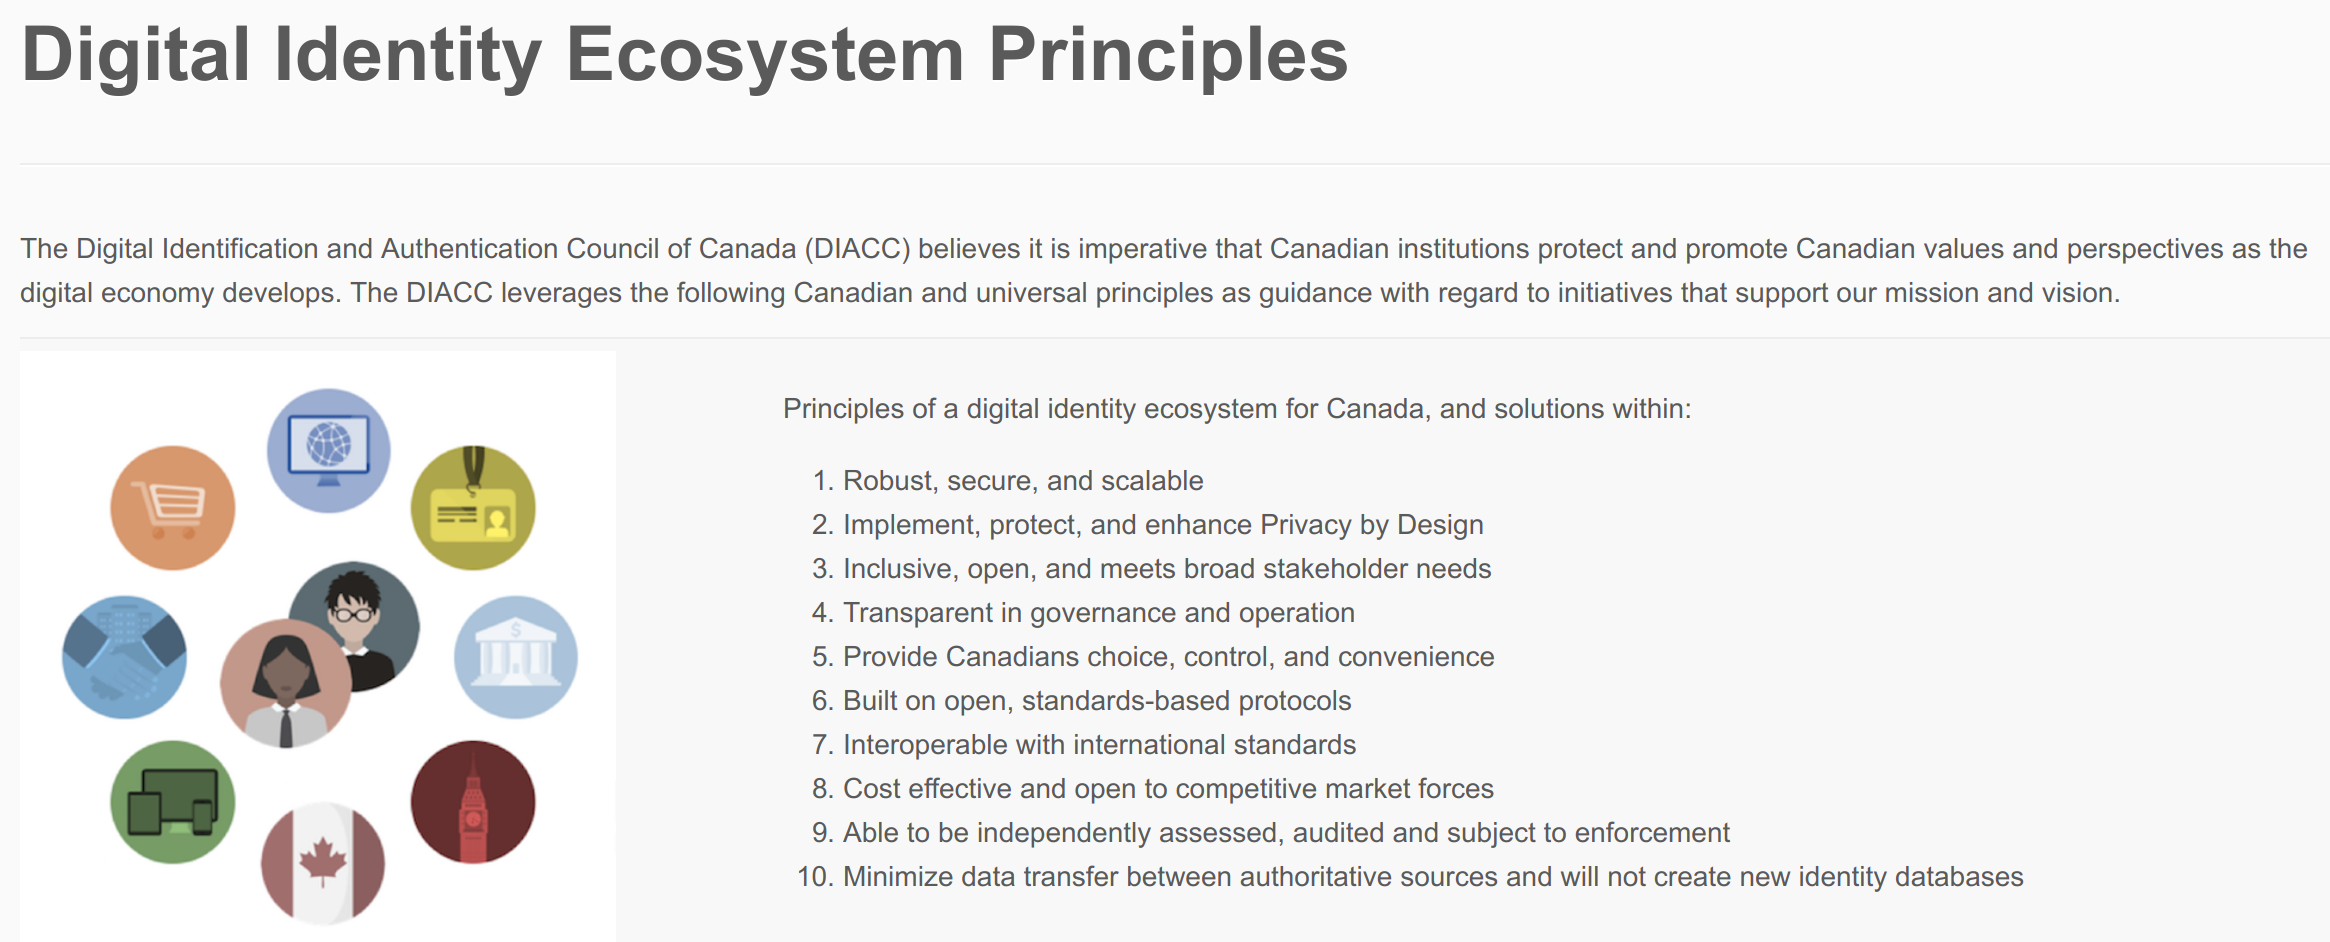
\includegraphics[width=12cm]{../pics/identity/diaac-principles}
	\end{figure}
}

\frame{
	\frametitle{Pan-Canadian Trust Framework | Cadre de Confiance pancanadien}
	\framesubtitle{\url{https://canada-ca.github.io/PCTF-CCP/}}
	\begin{figure}
		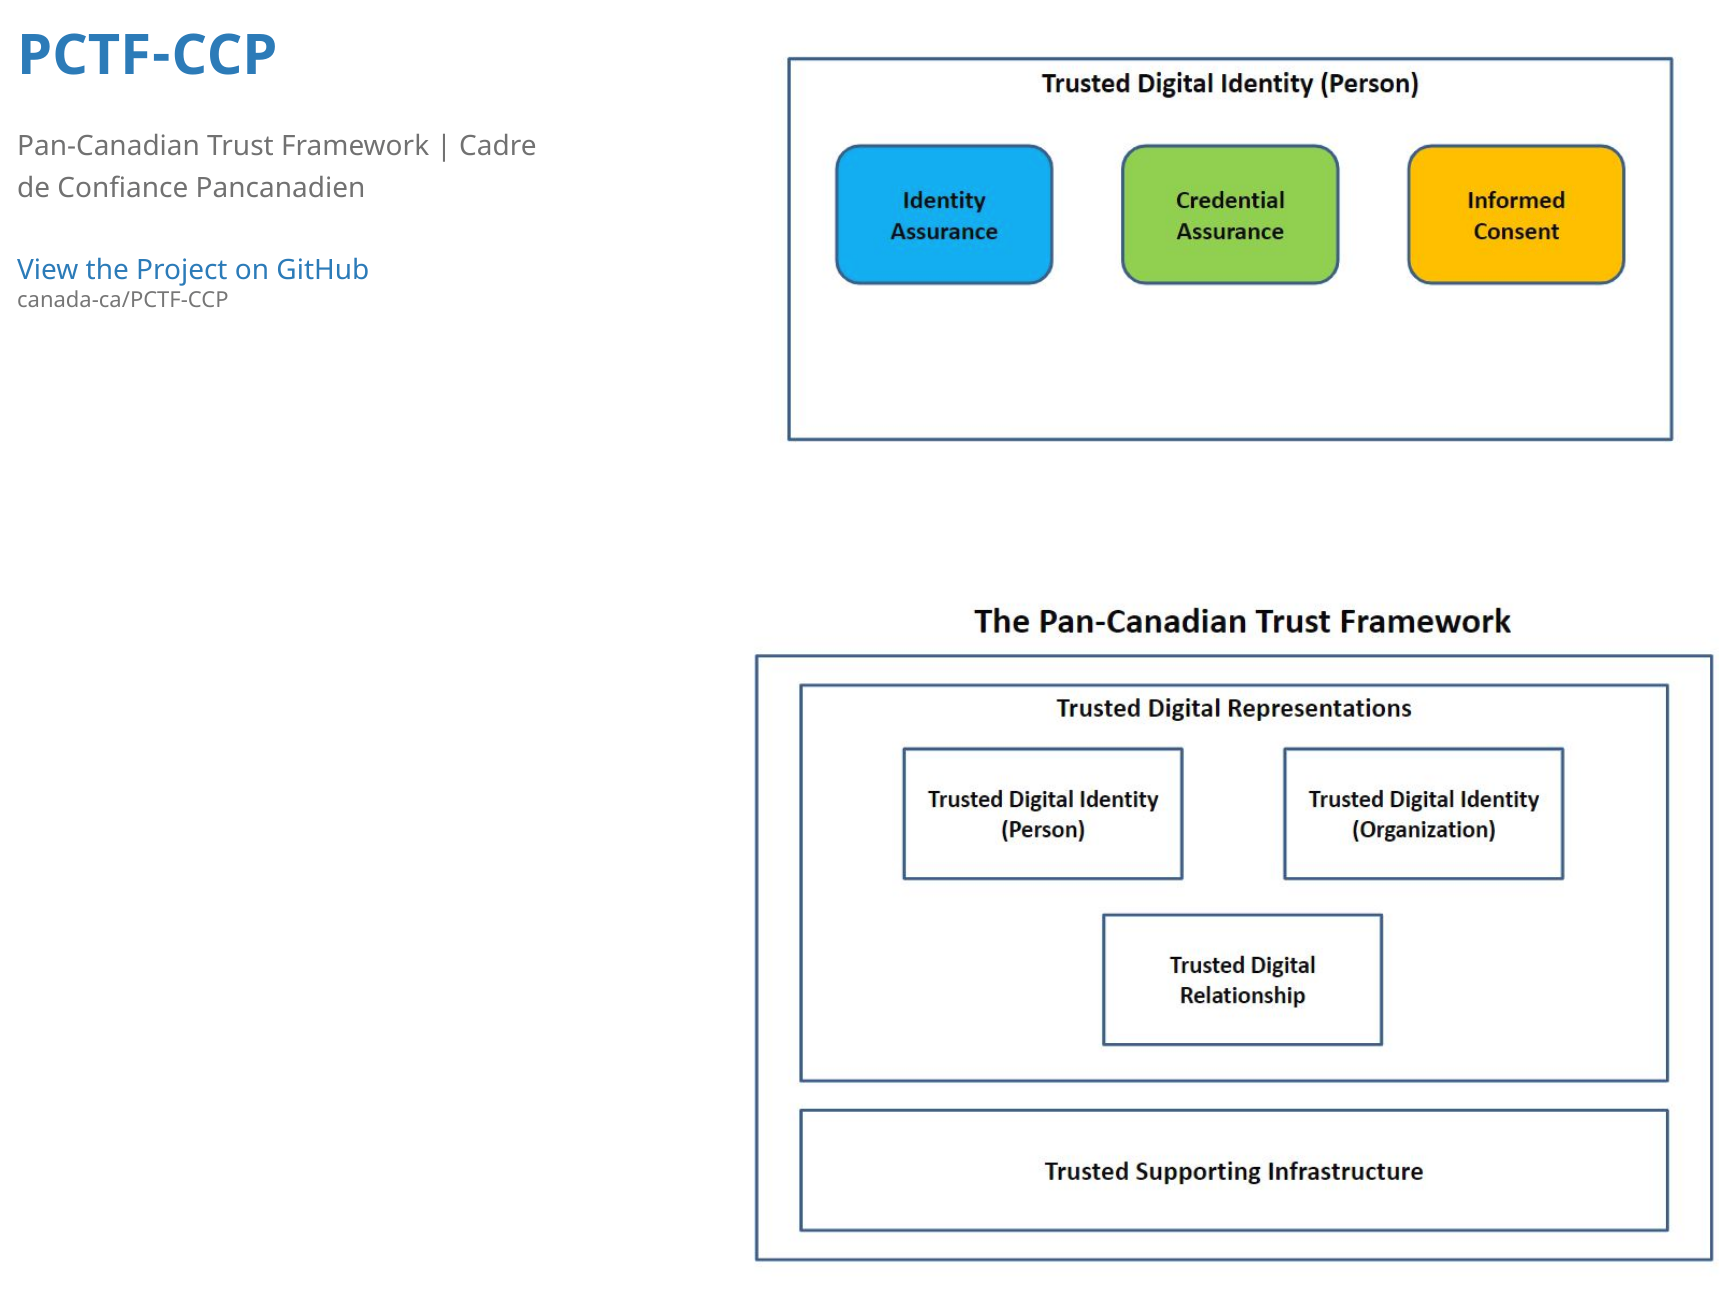
\includegraphics[height=6cm]{../pics/identity/pctf}
	\end{figure}
}

% ======================================================================================================
%                          Solutions providers
% ======================================================================================================
\section{Some Solutions Provider}

% --------------------------------------------------------------------------------------------------------
\subsection{Shyft Network}
\frame{
	\frametitle{Shyft Network}
	\framesubtitle{\url{https://shyft.network}}
	\begin{figure}
		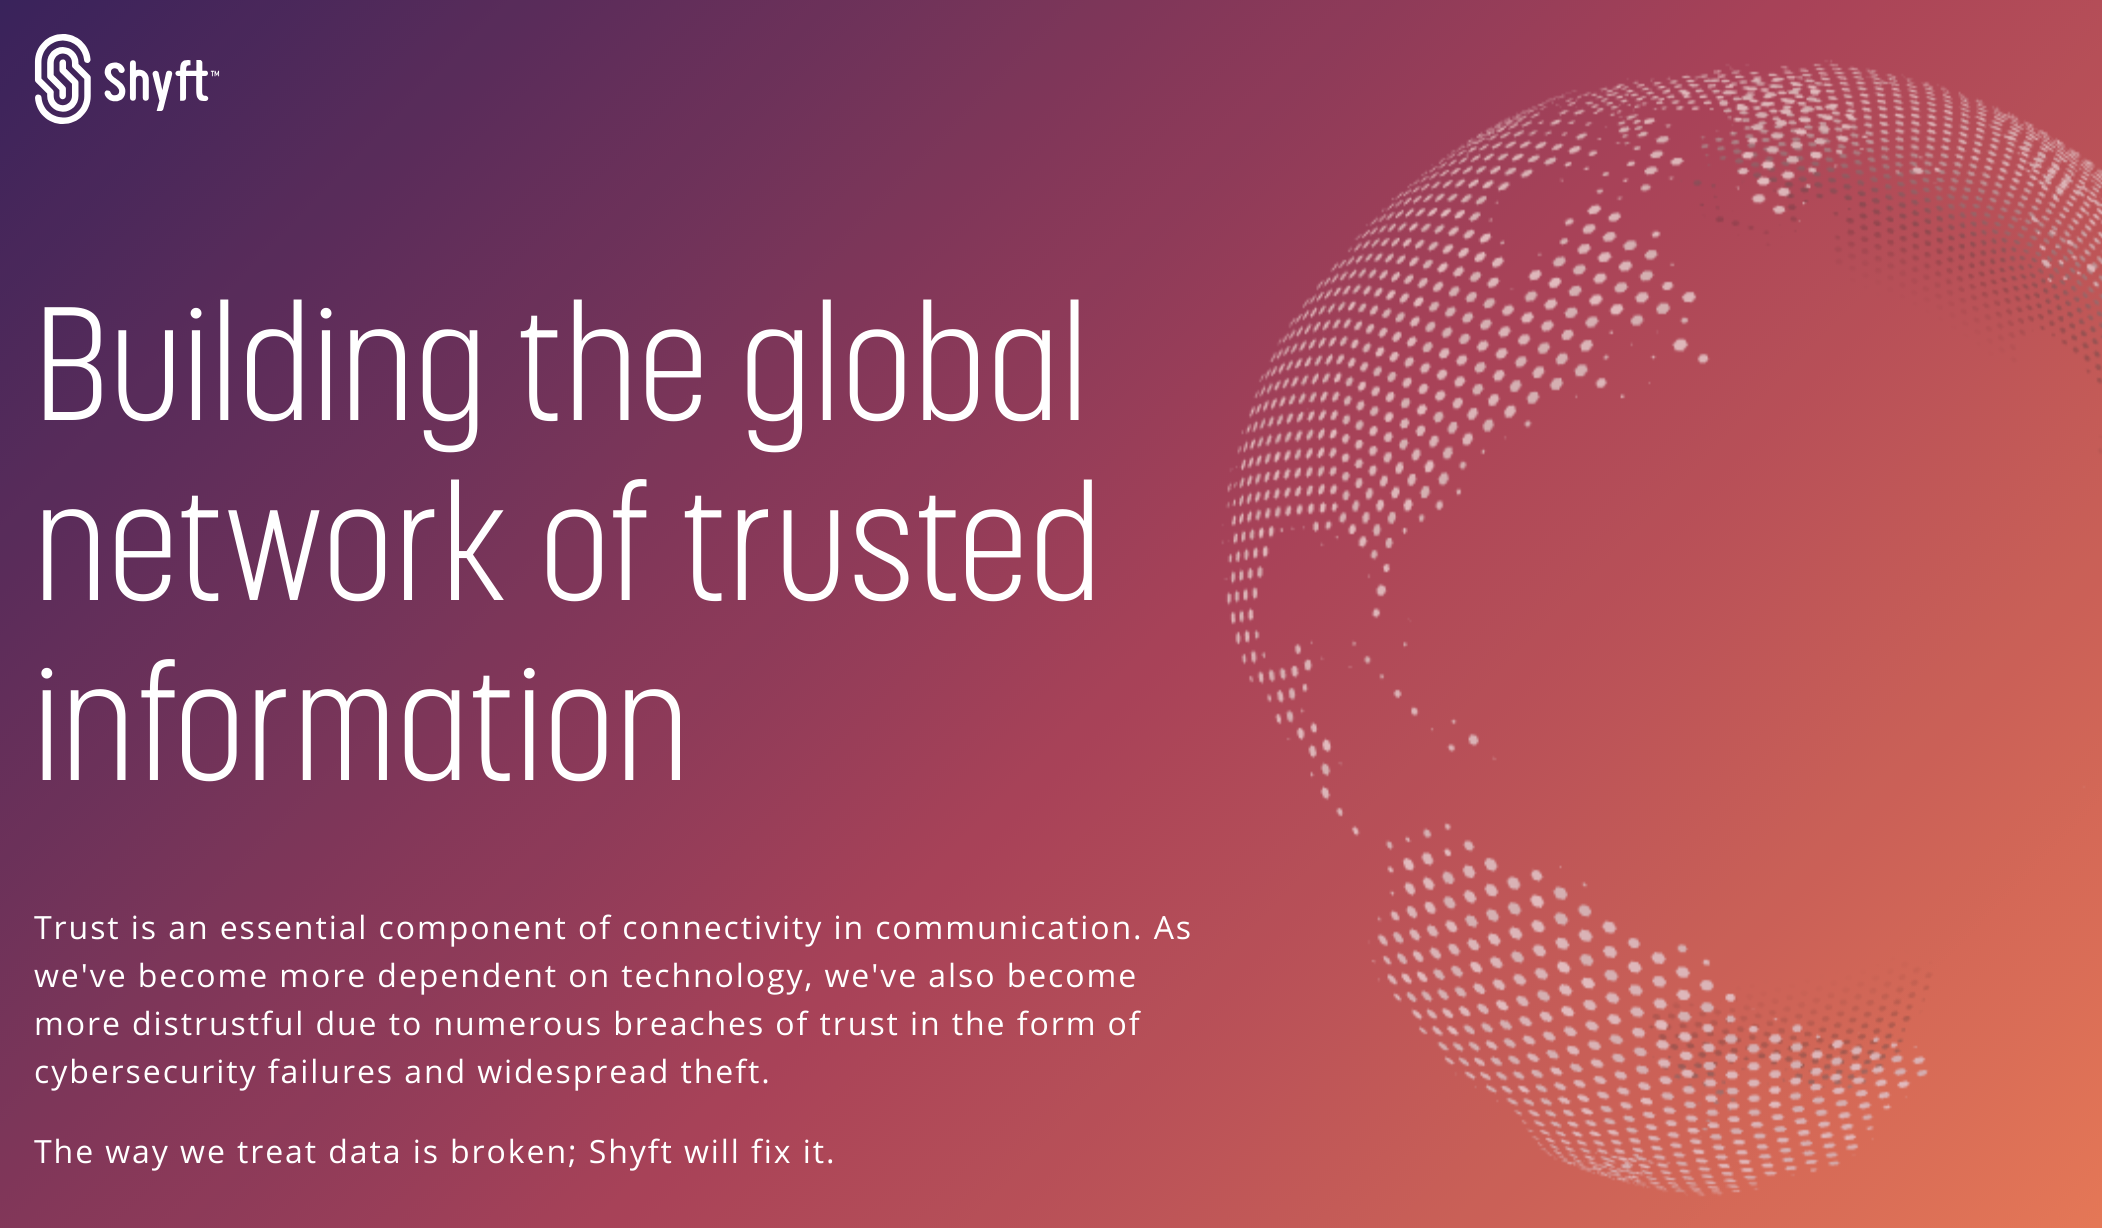
\includegraphics[height=6cm]{../pics/identity/shyft-home2}
	\end{figure}
}
% 2018-02	https://www.newswire.ca/news-releases/shyft-introduces-revolutionary-blockchain-based-kycaml-network-for-global-economy-673363883.html
% 2018-05	https://www.shyft.network/blog/2018/05/15/shyft-signs-mou-with-the-government-of-bermuda-pledges-to-invest-dollar10m-in-education-and-economic-development
% 2018-06	https://www.shyft.network/blog/2018/06/26/shyft-enters-program-partnership-with-pegasus-fintech-and-crypto-kabn
% 2018-08	https://www.globenewswire.com/news-release/2018/08/16/1553166/0/en/Shyft-Engages-First-Group-of-Trust-Anchors-With-Over-One-Billion-Data-Points-To-Network-and-Rolls-Out-TestNet.html
% 2018-12	https://medium.com/shyft-network-media/shyft-partners-with-bitt-to-enable-a-private-and-secure-data-ecosystem-for-barbados-and-the-955652da4471
% 2019-03	https://ncfacanada.org/polymath-and-kabn-announce-consortium-to-accelerate-the-creation-distribution-and-management-of-digital-securities-across-multiple-jurisdictions-and-platforms/


% --------------------------------------------------------------------------------------------------------
\subsection{Evernym / Sovrin / Indy}
\frame{
	\frametitle{Evernym / Sovrin / Indy}
	\framesubtitle{\url{https://www.evernym.com}, \url{https://sovrin.org}, and \url{https://www.hyperledger.org/projects/hyperledger-indy}}
%	\begin{block}
%	The Sovrin Foundation is a 501 (c)(4) nonprofit organization established to administer the Governance Framework governing the Sovrin Network, a public service utility enabling self-sovereign identity on the internet. The Sovrin Foundation is an independent organization that is responsible for ensuring the Sovrin identity system is public and globally accessible.
%	\end{block}
	\begin{figure}
		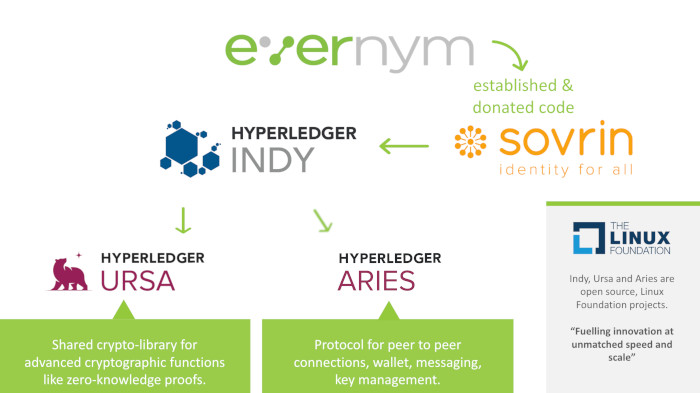
\includegraphics[height=6cm]{../pics/identity/evernym-sovrin-hyperledger-aries}
	\end{figure}
	\centering
	Try it at \url{https://try.connect.me} 
}

% --------------------------------------------------------------------------------------------------------
\subsection{uPort}
\frame{
	\frametitle{uPort}
	\framesubtitle{\url{https://www.uport.me}}
	\begin{figure}
		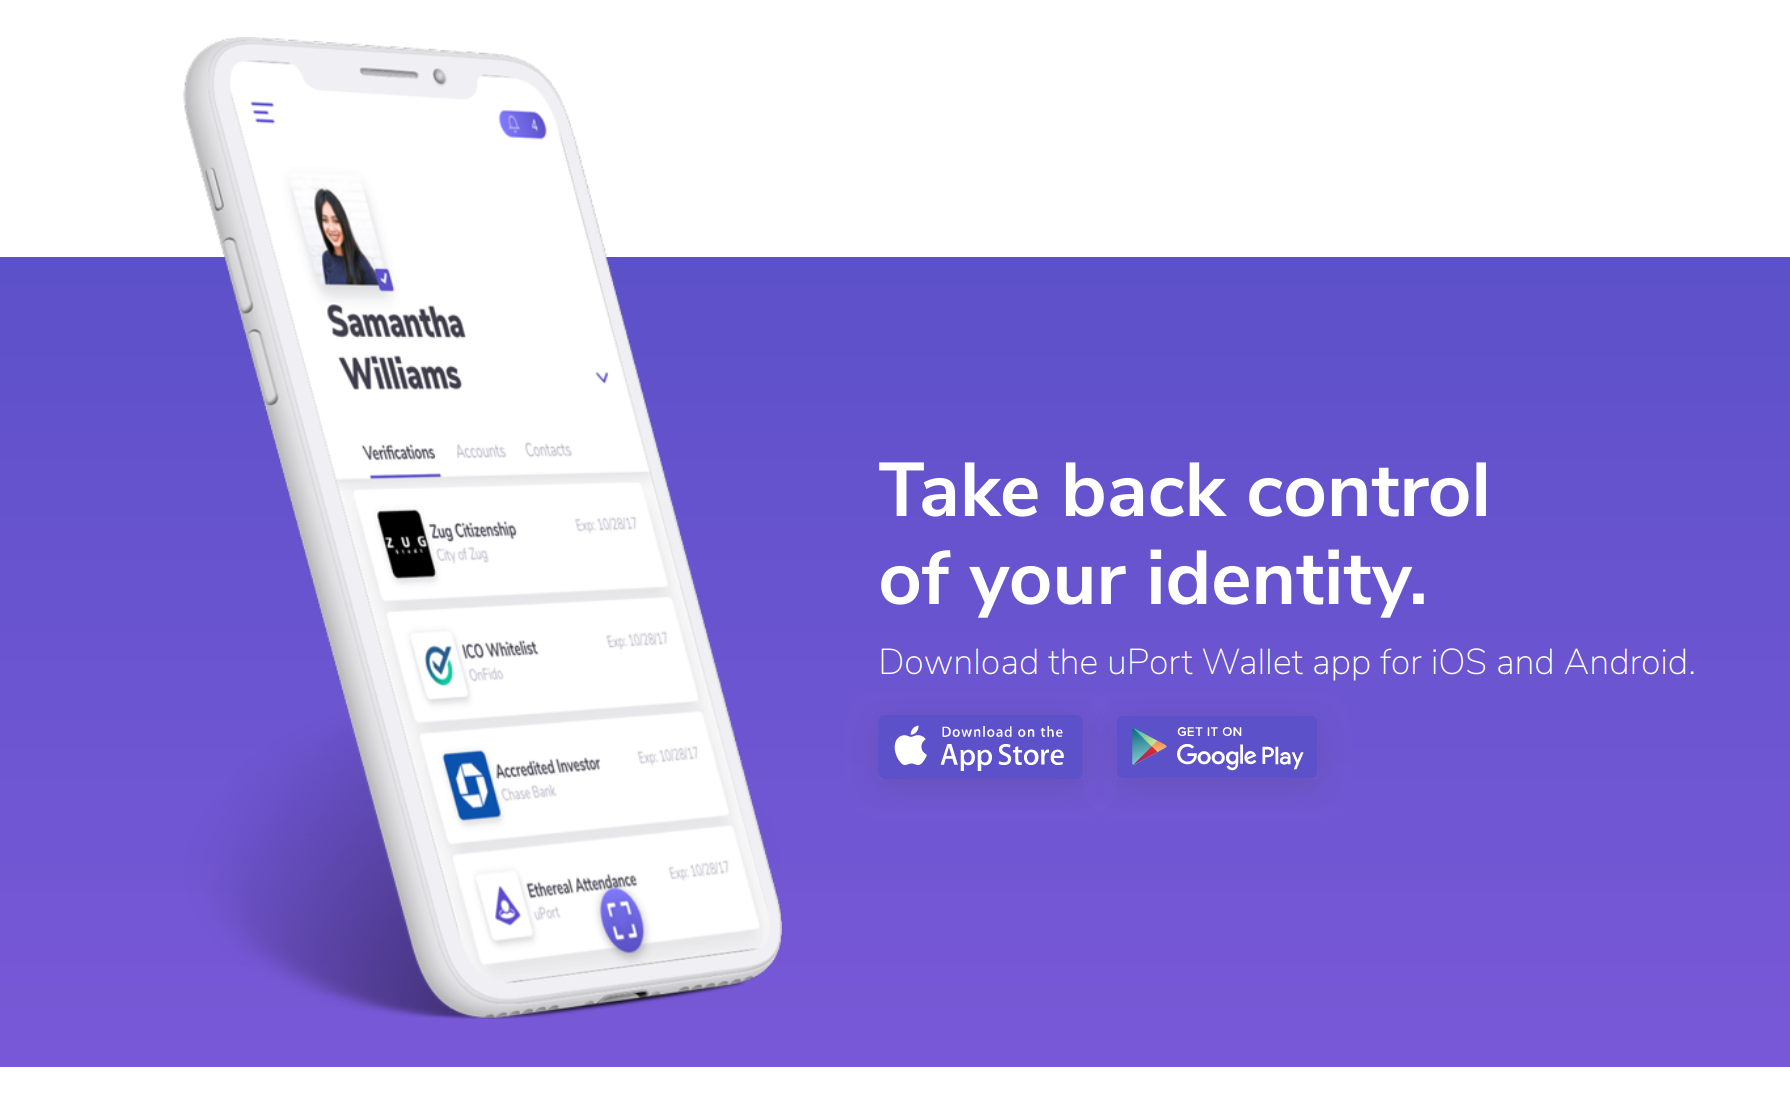
\includegraphics[height=6cm]{../pics/identity/uPort-app}
	\end{figure}
	\centering
	Try it at \url{https://uportlandia.uport.me}
}


% --------------------------------------------------------------------------------------------------------
\subsection{SecureKey}
\frame{
	\frametitle{SecureKey}
	\framesubtitle{\url{https://securekey.com}}
	\begin{figure}
		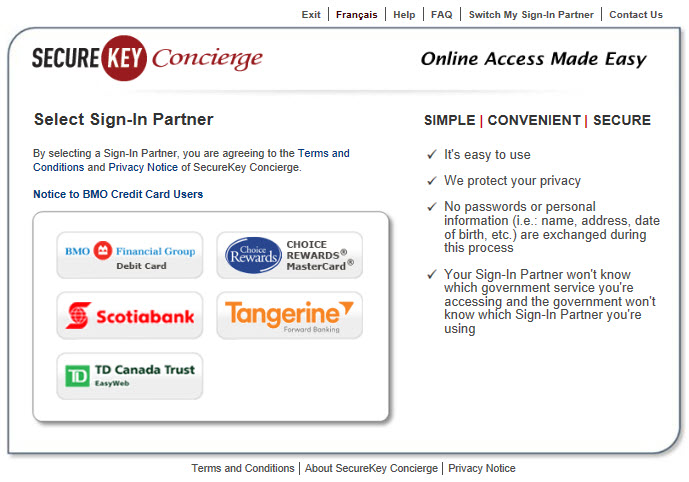
\includegraphics[height=6cm]{../pics/identity/securekey-EG-PartnerSign-In-EN}
		\captionsetup{justification=centering}
	\end{figure}
}
	
% --------------------------------------------------------------------------------------------------------
\subsection{Microsoft ION}
\frame{
	\frametitle{Microsoft ION}
	\framesubtitle{\url{https://github.com/decentralized-identity/ion}}
	\begin{figure}
		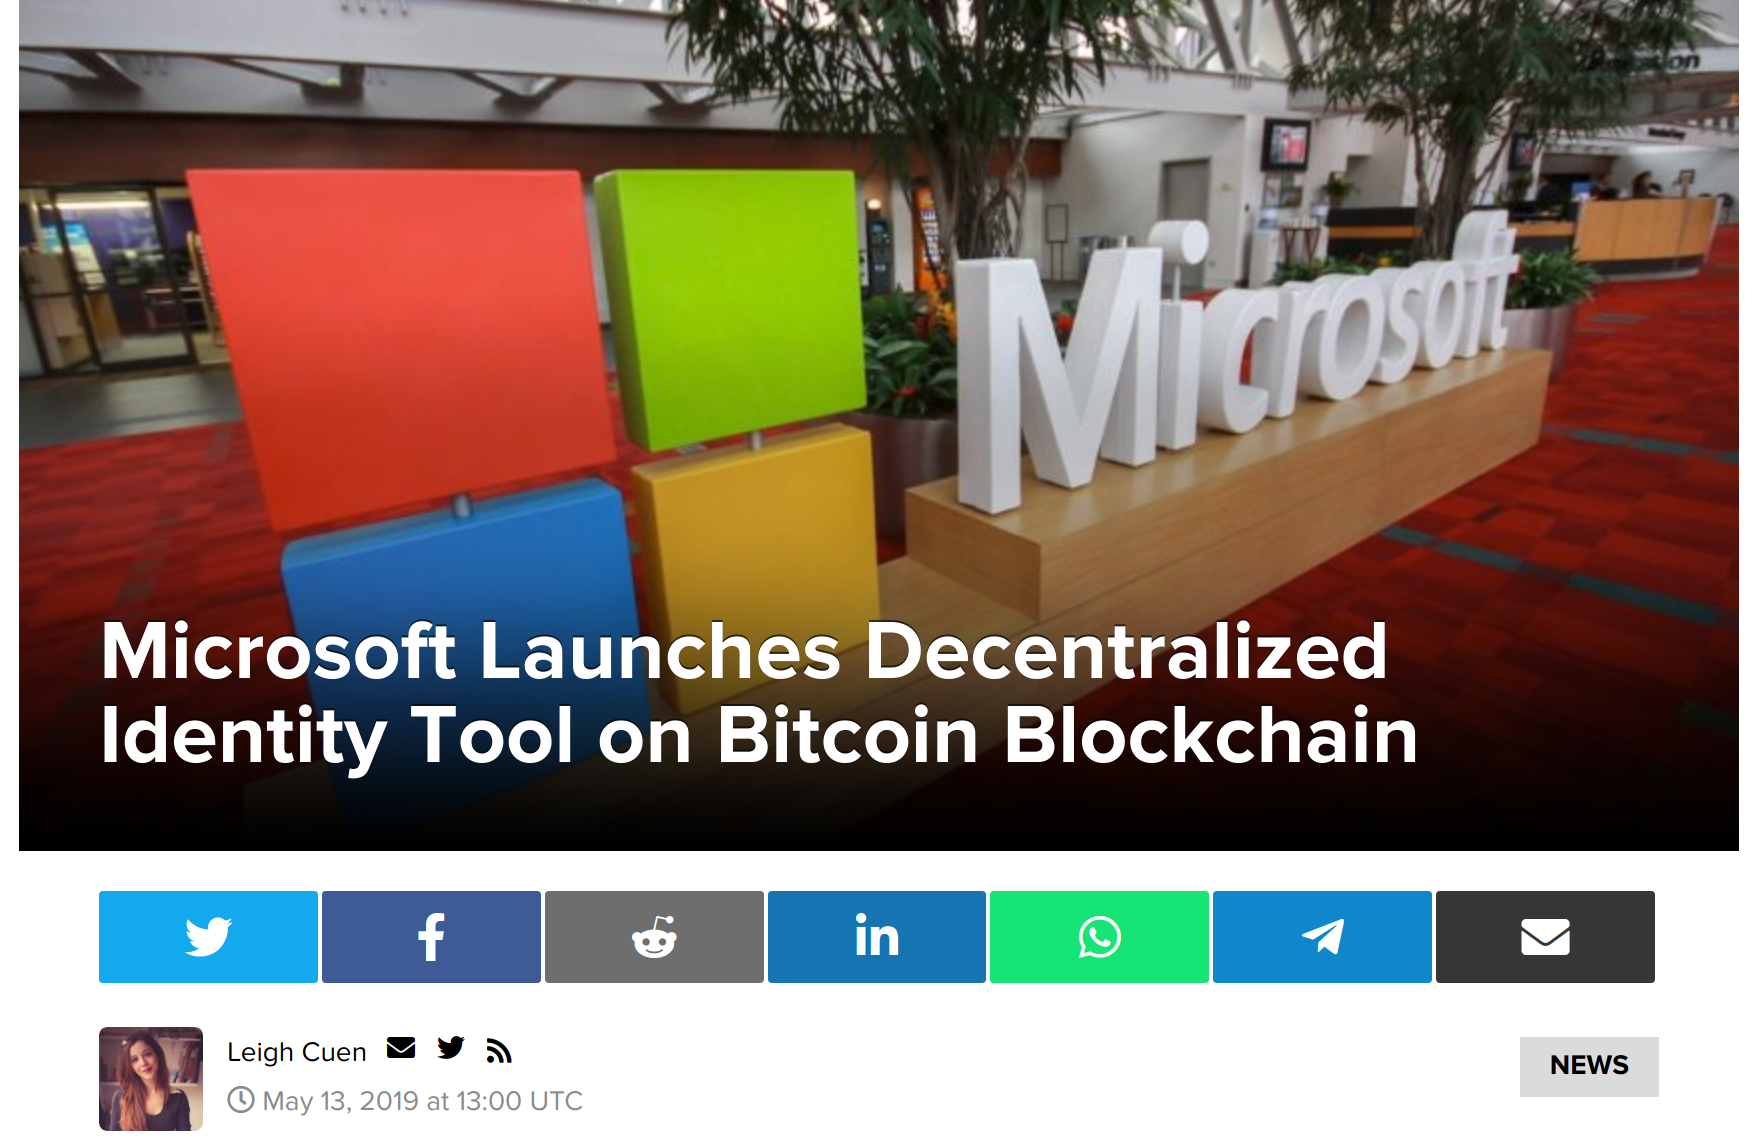
\includegraphics[height=6cm]{../pics/identity/leighcuen-msft-ion}
		\captionsetup{justification=centering}
		\caption{from \cite{leighcuen20190513-ion}}
	\end{figure}
}
	

% --------------------------------------------------------------------------------------------------------
\subsection{KABN}
\frame{
	\frametitle{KABN --- Blockchain Identity}
	\framesubtitle{\url{https://medium.com/@secdegulleri/kabn-blockchain-identity-daf70ee0eb4}}
	\begin{figure}
		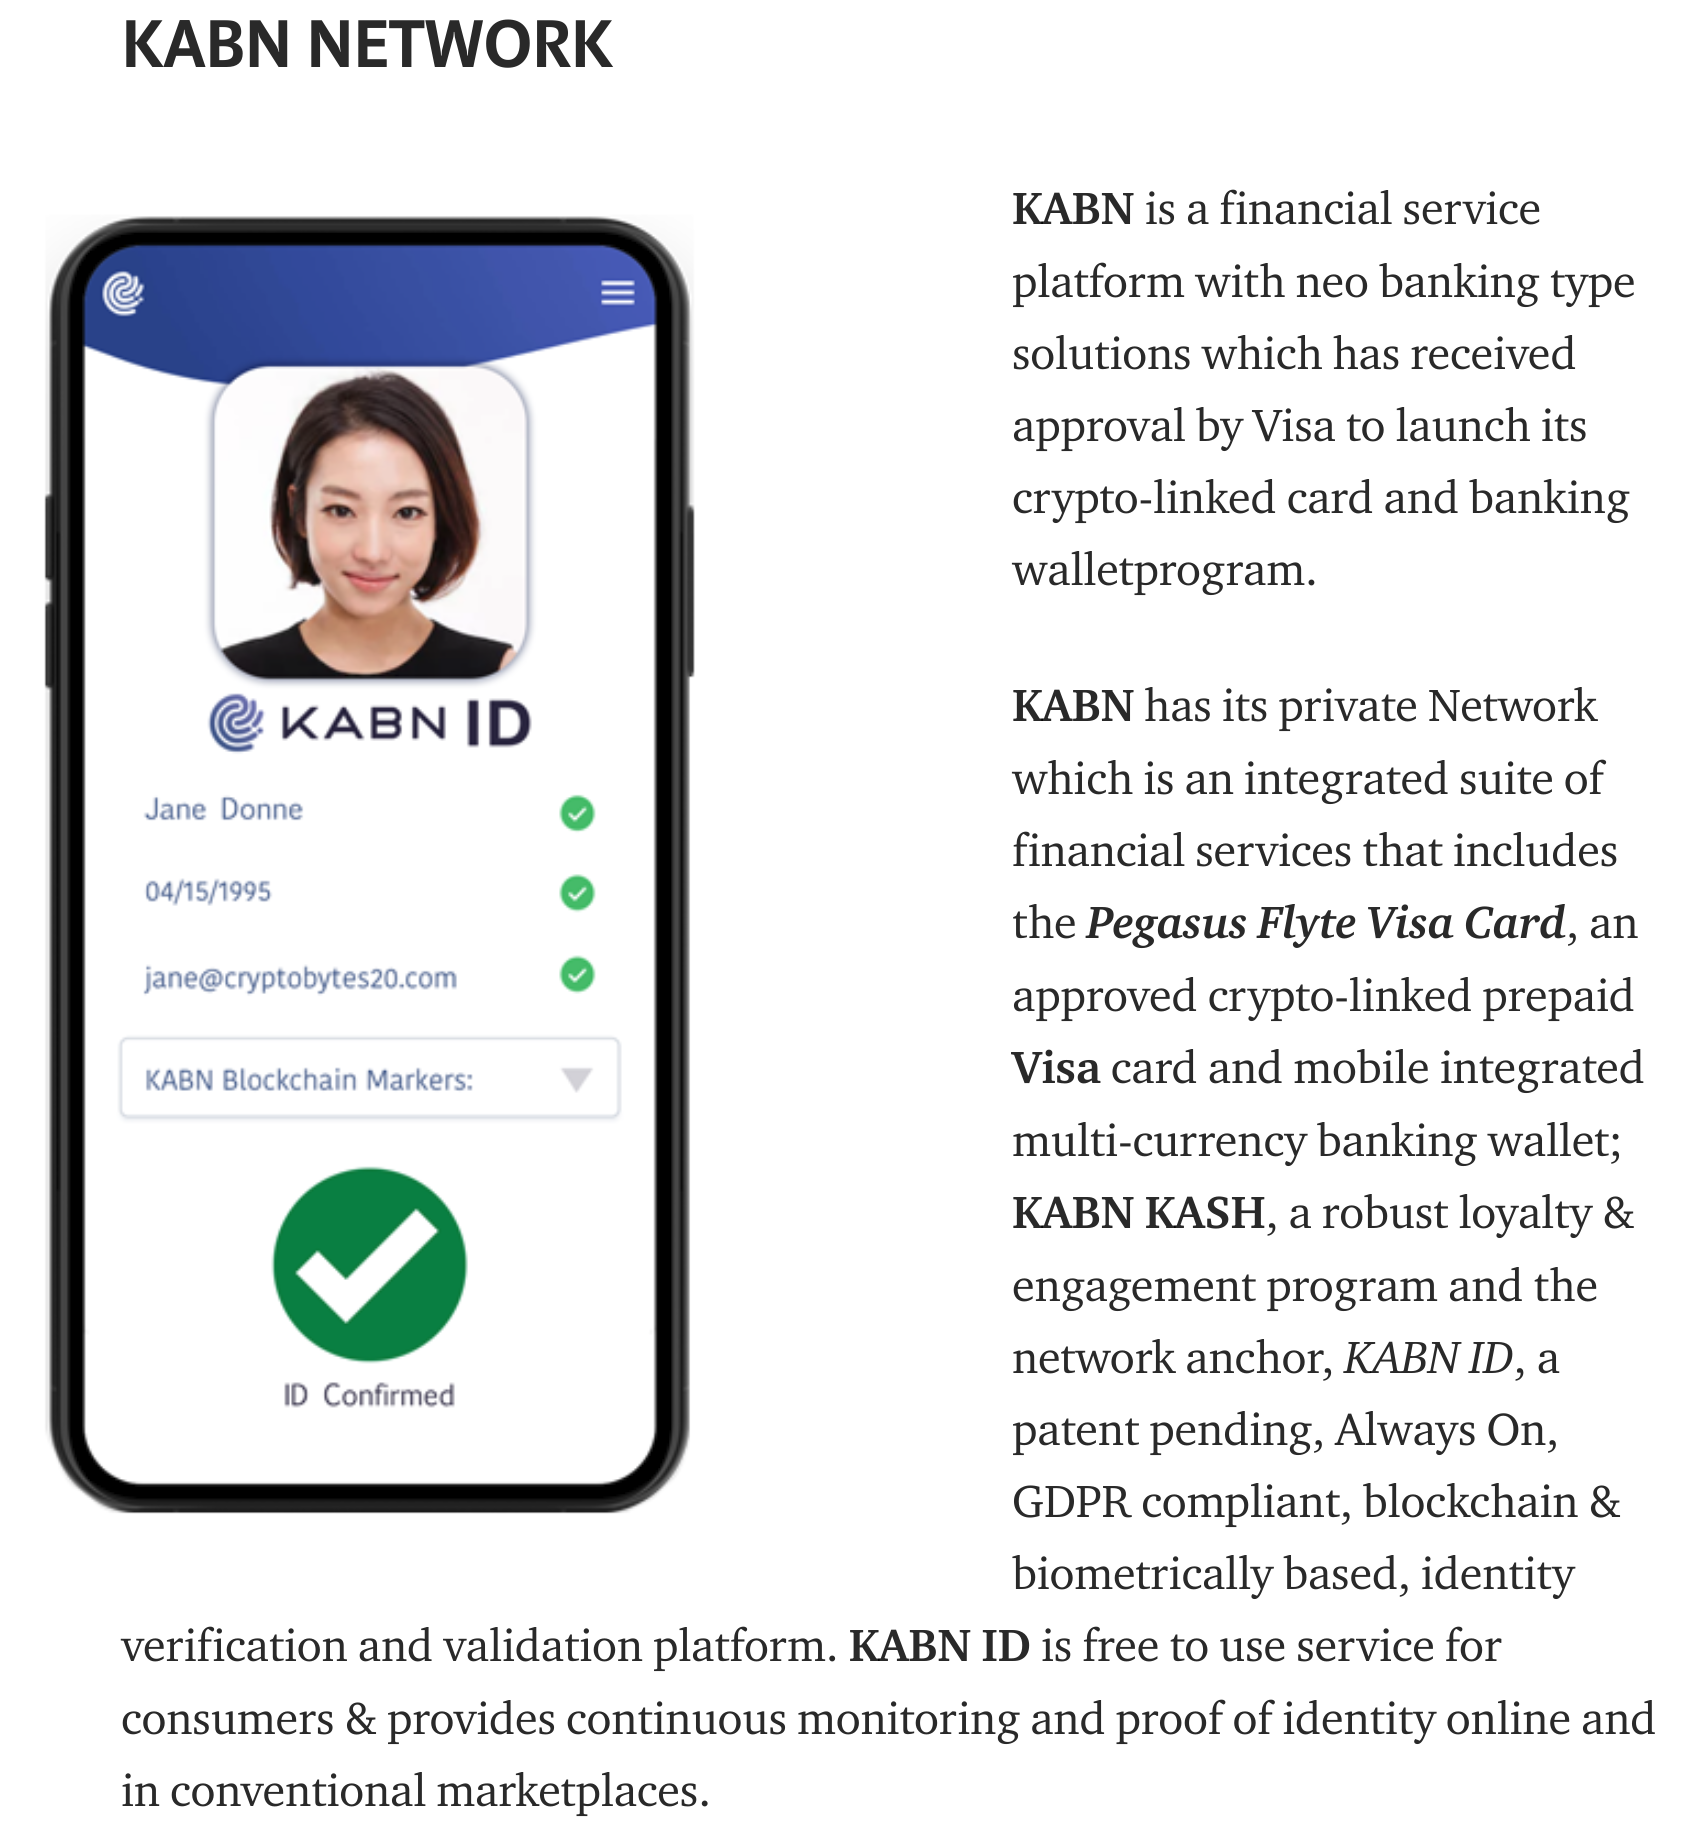
\includegraphics[height=6cm]{../pics/identity/kabn}
	\end{figure}
}

%\frame{
%	\frametitle{Polymath and KABN consortium announcement}
%	\framesubtitle{\url{https://ncfacanada.org/polymath-and-kabn-announce-consortium-to-accelerate-the-creation-distribution-and-management-of-digital-securities-across-multiple-jurisdictions-and-platforms/}}
%	\begin{figure}
%		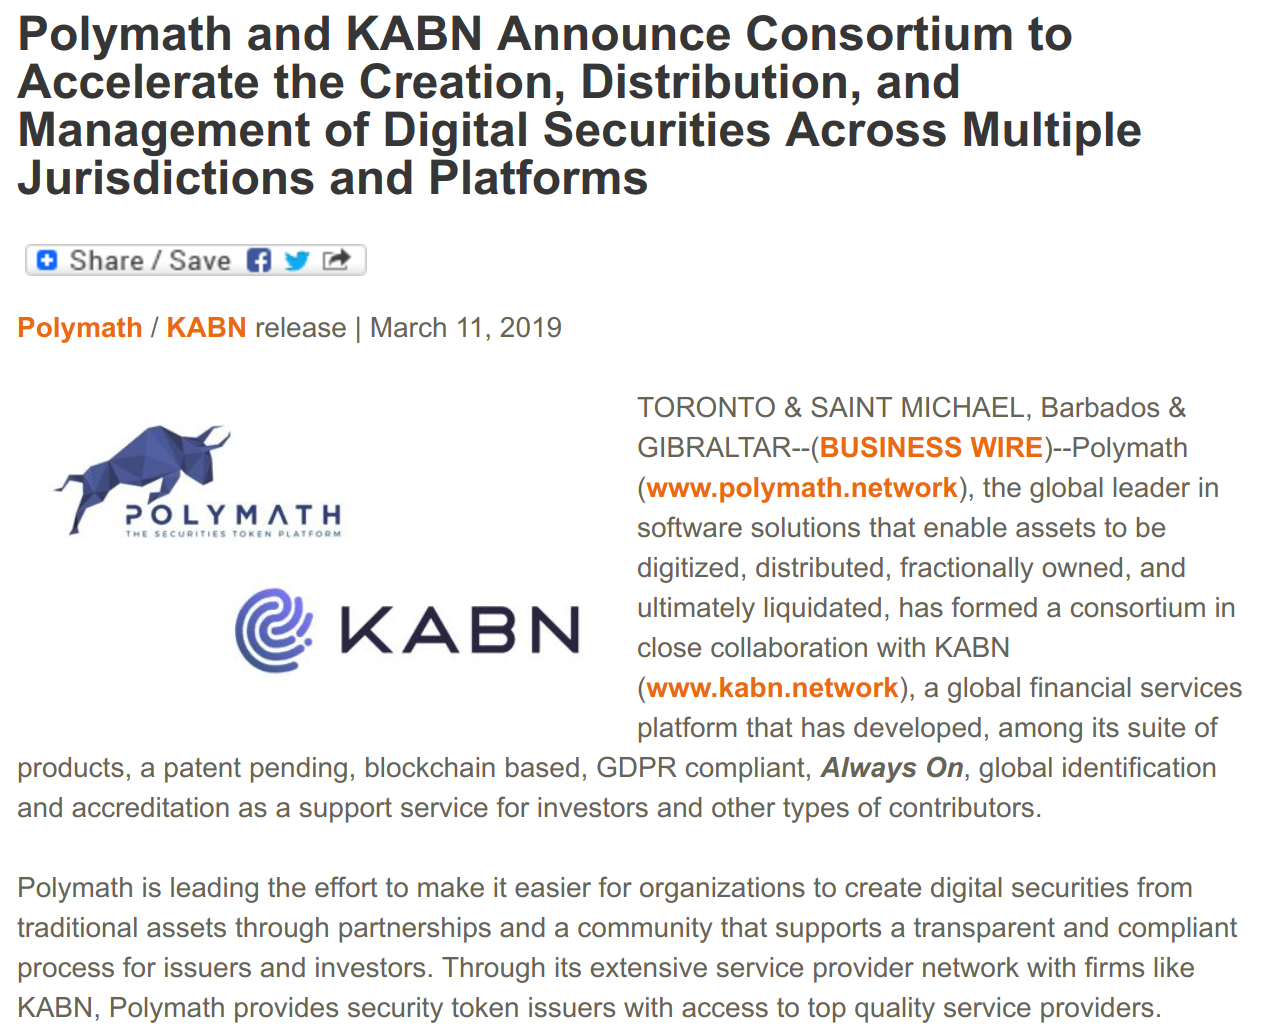
\includegraphics[height=6cm]{../pics/identity/polymath-kabn}
%	\end{figure}
%}



% ======================================================================================================
%                          Examples of application in industry
% ======================================================================================================
\section{Case Studies}

\subsection{Switzerland}
\frame{
	\frametitle{The first e-bike service worldwide powered by decentralized identity}
	\framesubtitle{See full article from \cite{nawfal2019:uport-bike}}
	% https://medium.com/uport/zug-residents-can-now-ride-e-bikes-using-their-uport-powered-zug-digital-ids-7ed31ac9d621
	% see also Zug eID launch -- https://www.ethnews.com/zug-and-uport-see-first-citizens-identity-registered-on-the-ethereum-blockchain
	\begin{figure}
		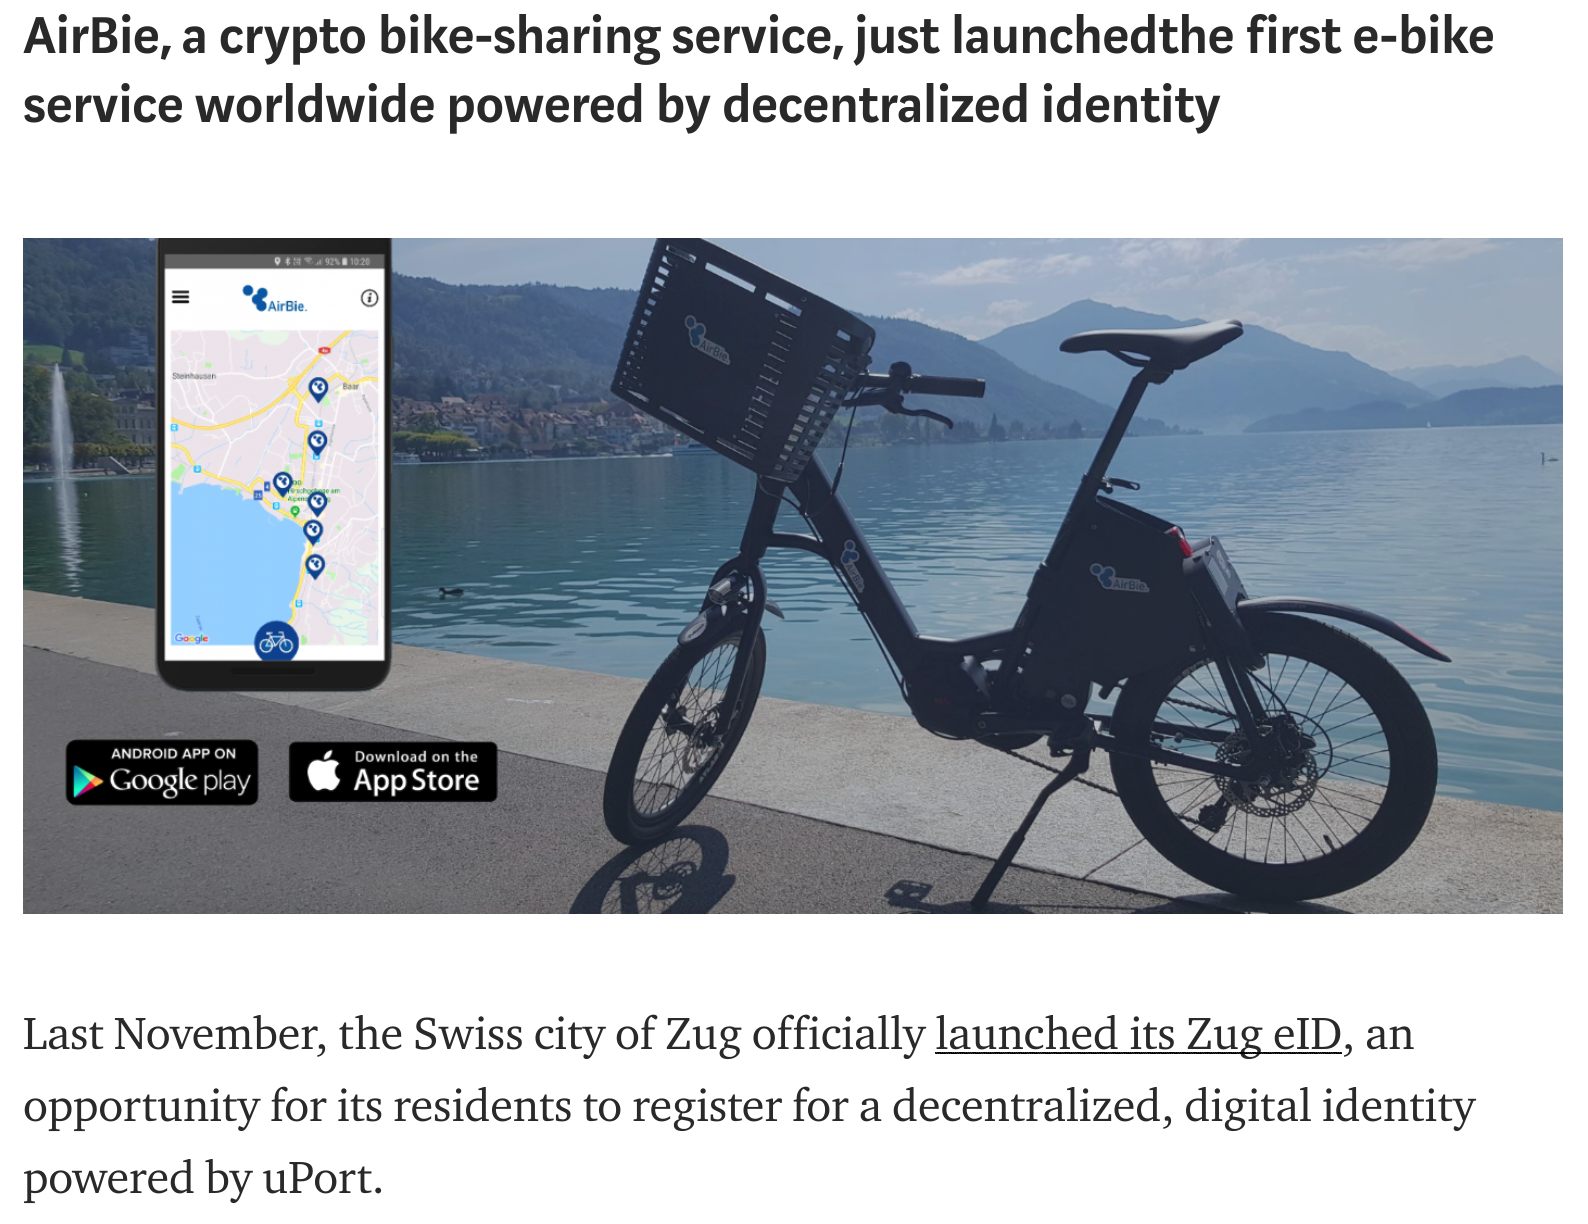
\includegraphics[height=6cm]{../pics/identity/uport-bike}
	\end{figure}
}

\subsection{Canada}
\frame{
	\frametitle{The Verifiable Organizations Network (VON)}
	\framesubtitle{\url{https://vonx.io}}
	\begin{figure}
		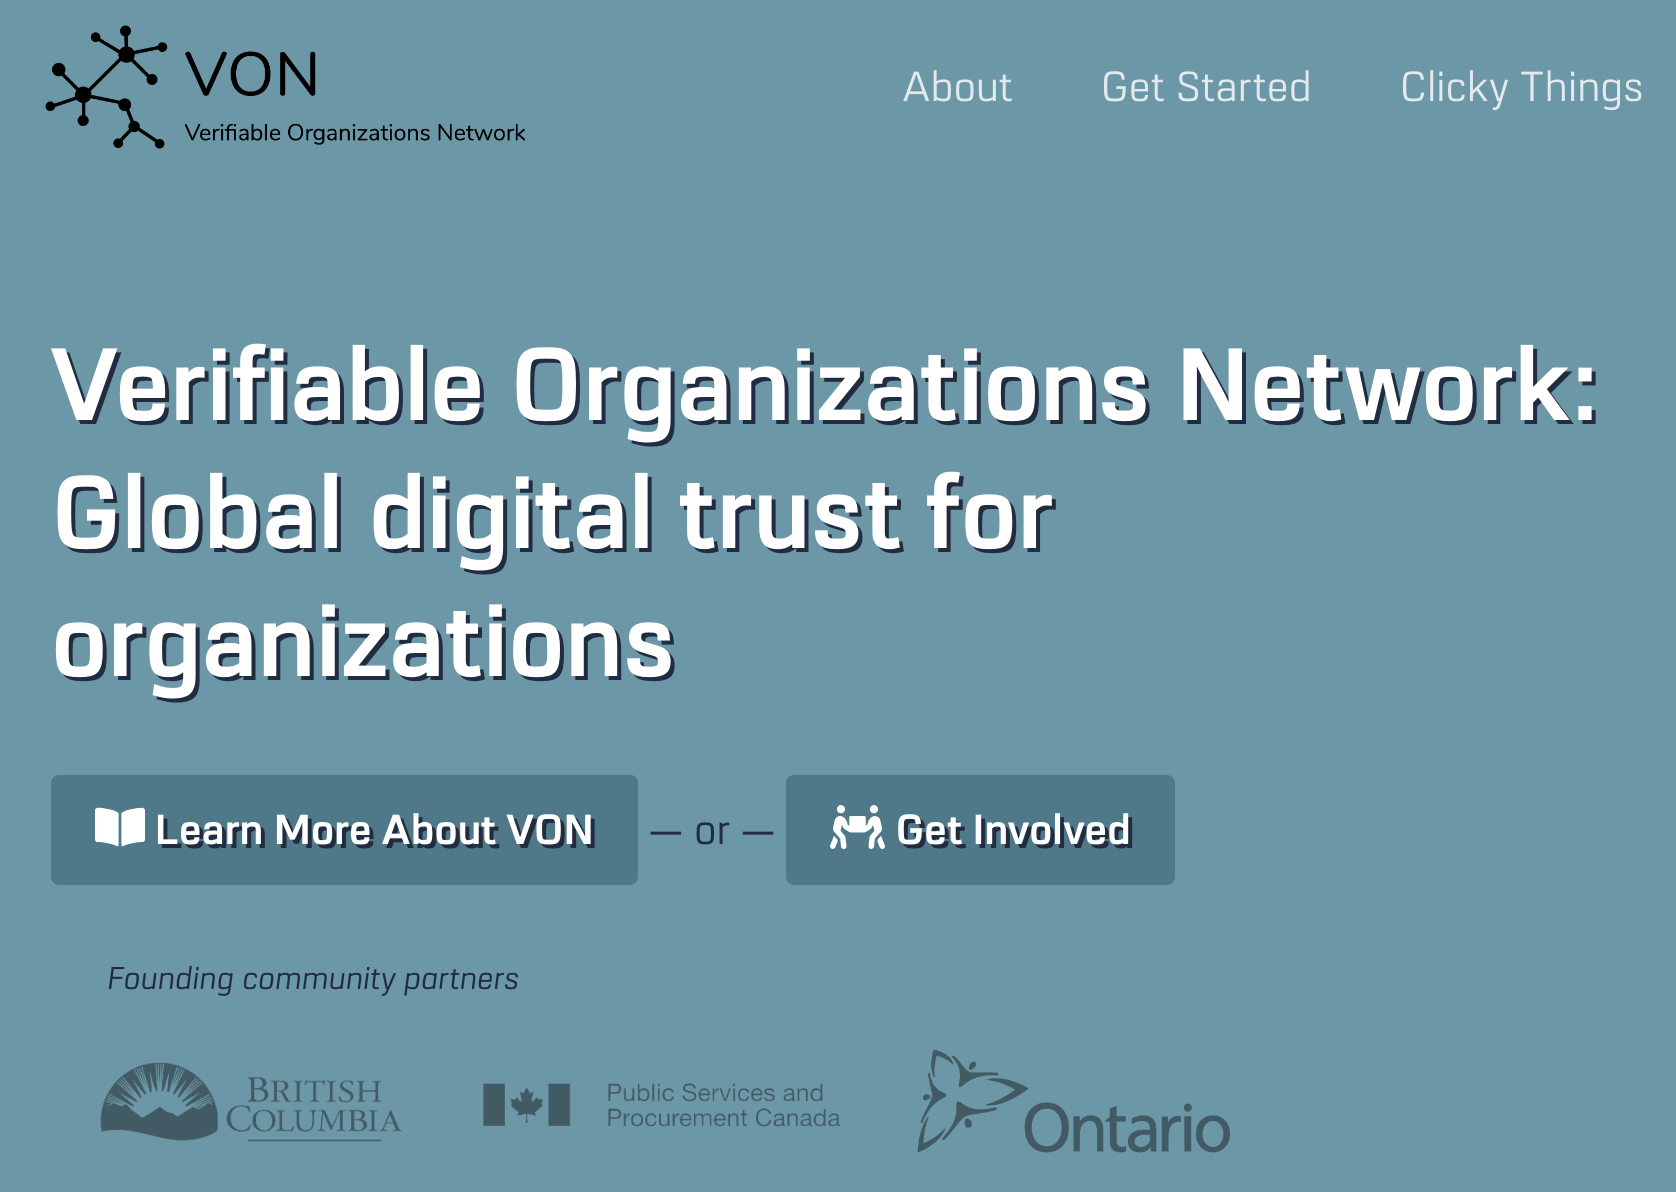
\includegraphics[height=6cm]{../pics/identity/vonx}
	\end{figure}
}

%\frame{
%	\frametitle{SSI in Alberta}
%	\begin{figure}
%		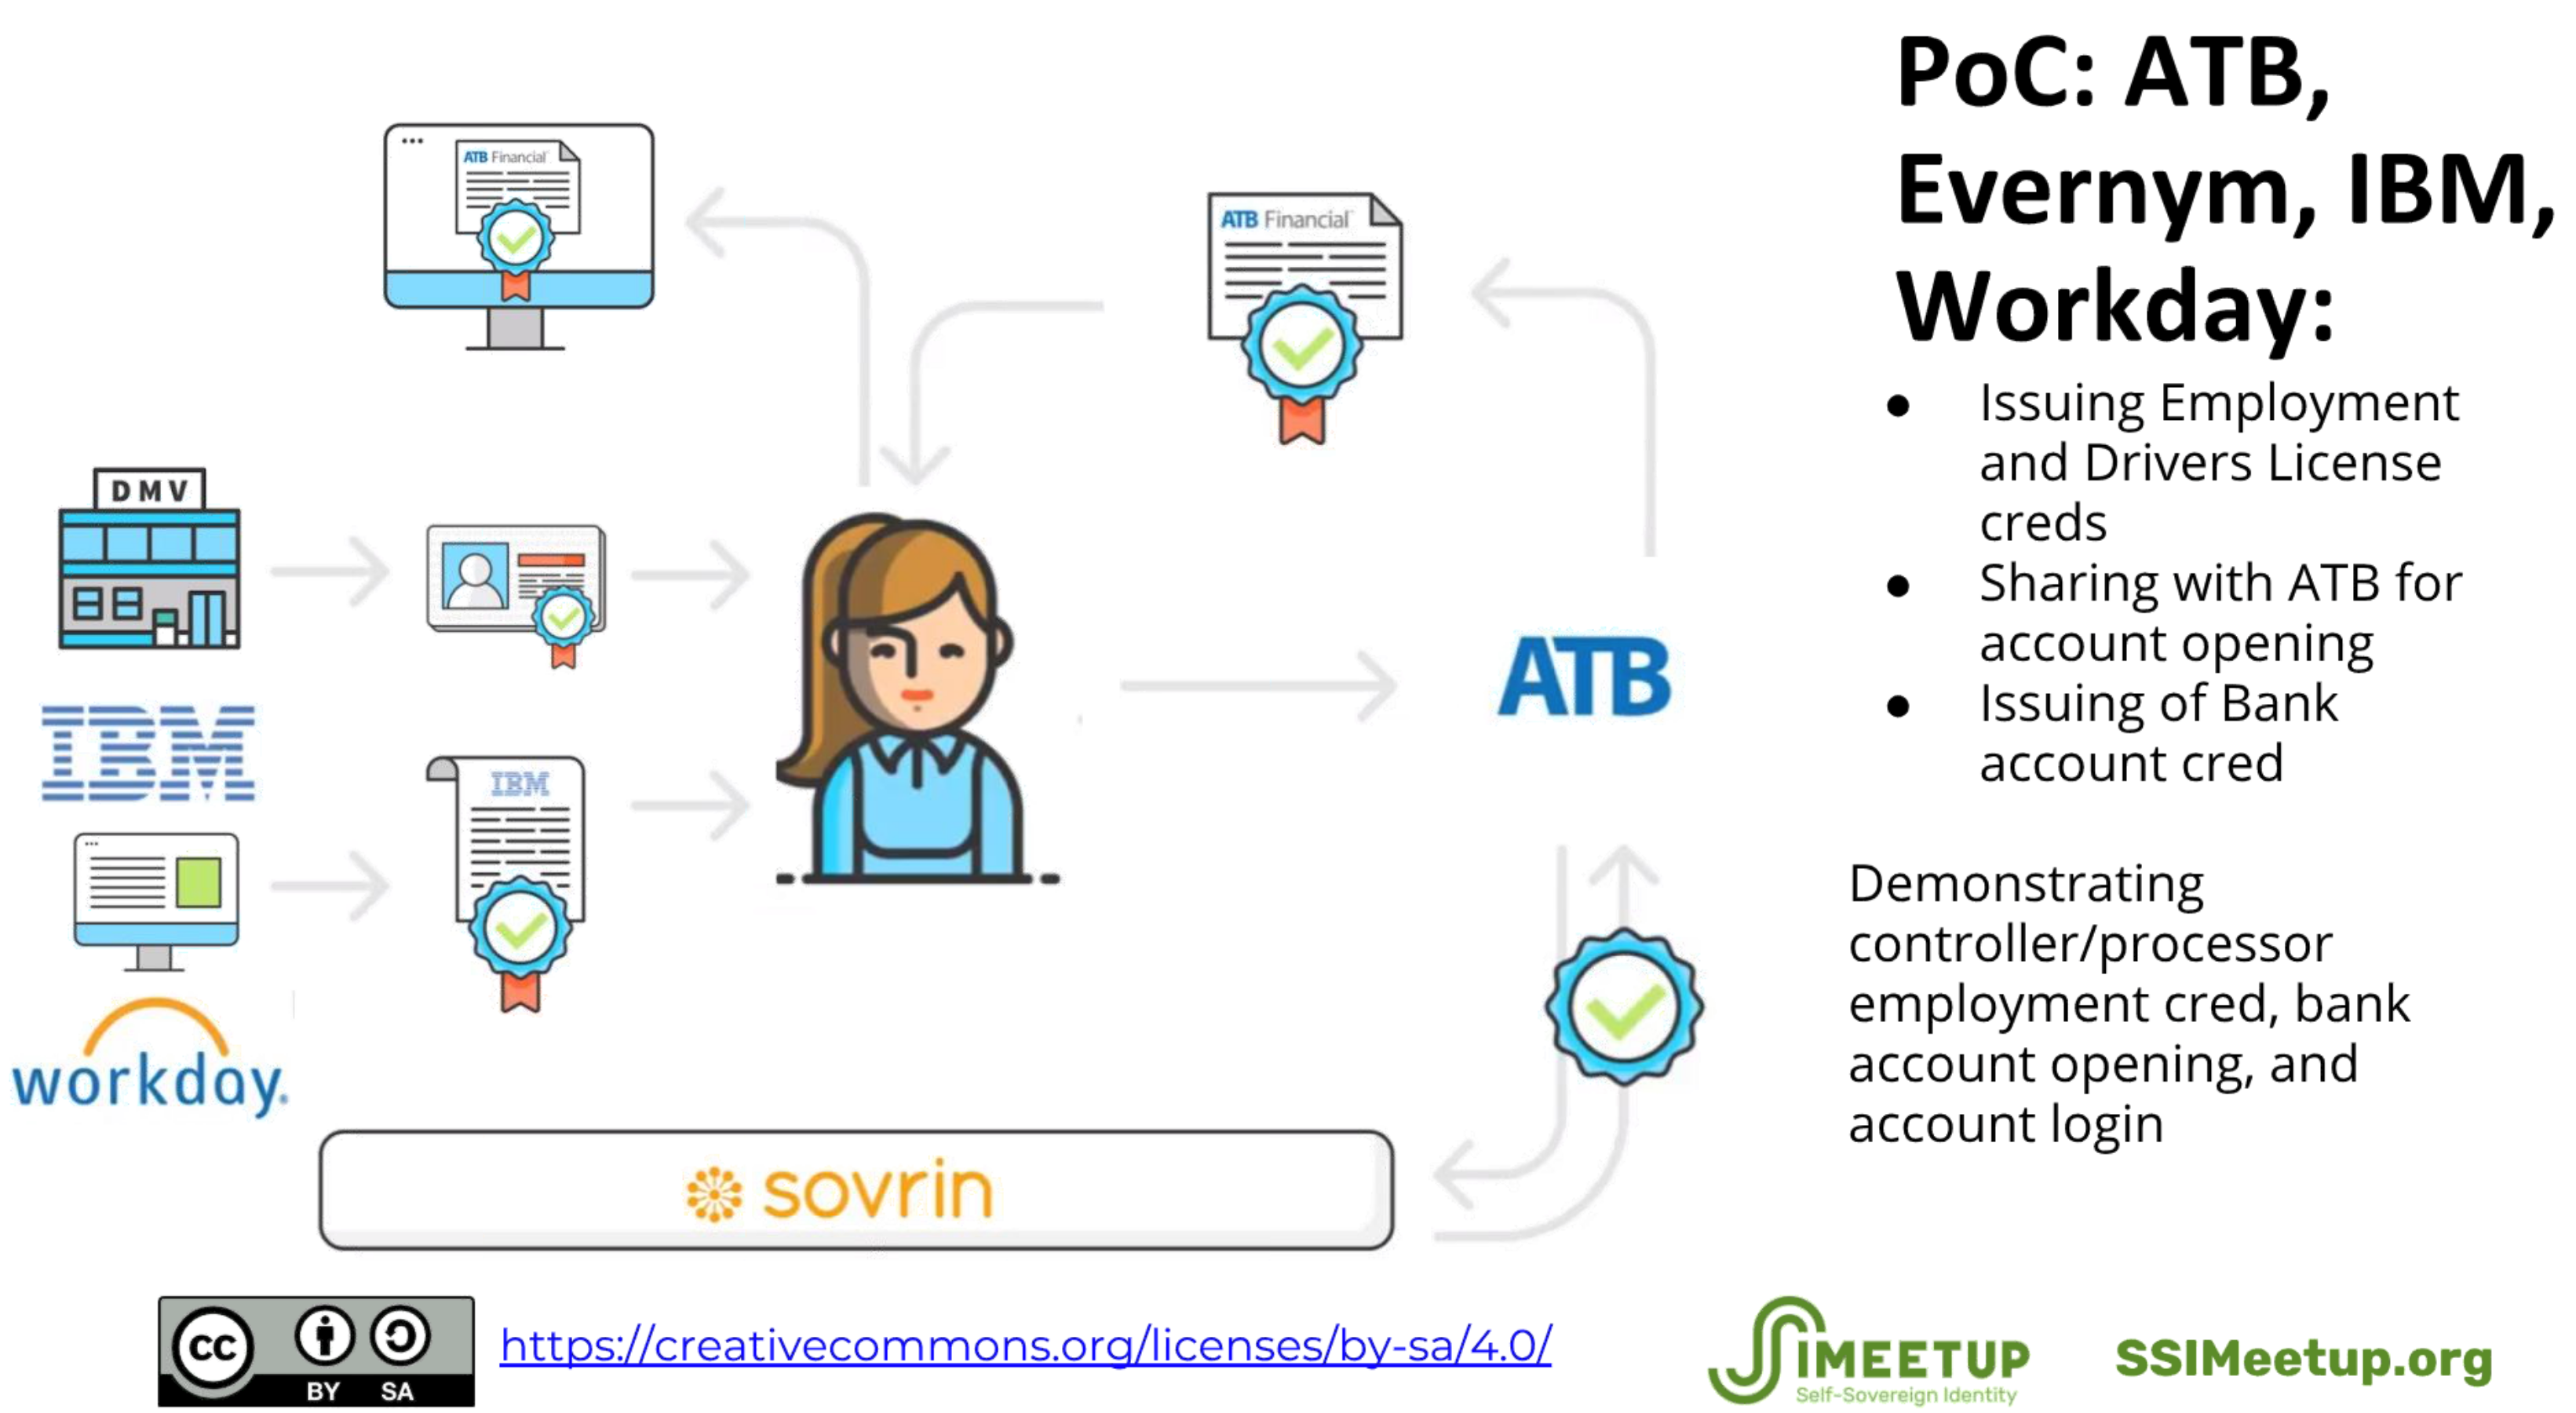
\includegraphics[height=6cm]{../pics/case_studies/atb-evernym-ibm-workday}
%		\captionsetup{justification=centering}
%		\caption{from \cite{ssimeetup201902:atb-slides}}
%	\end{figure}
%}

\frame{
	\frametitle{SSI in Alberta}
	\begin{figure}
		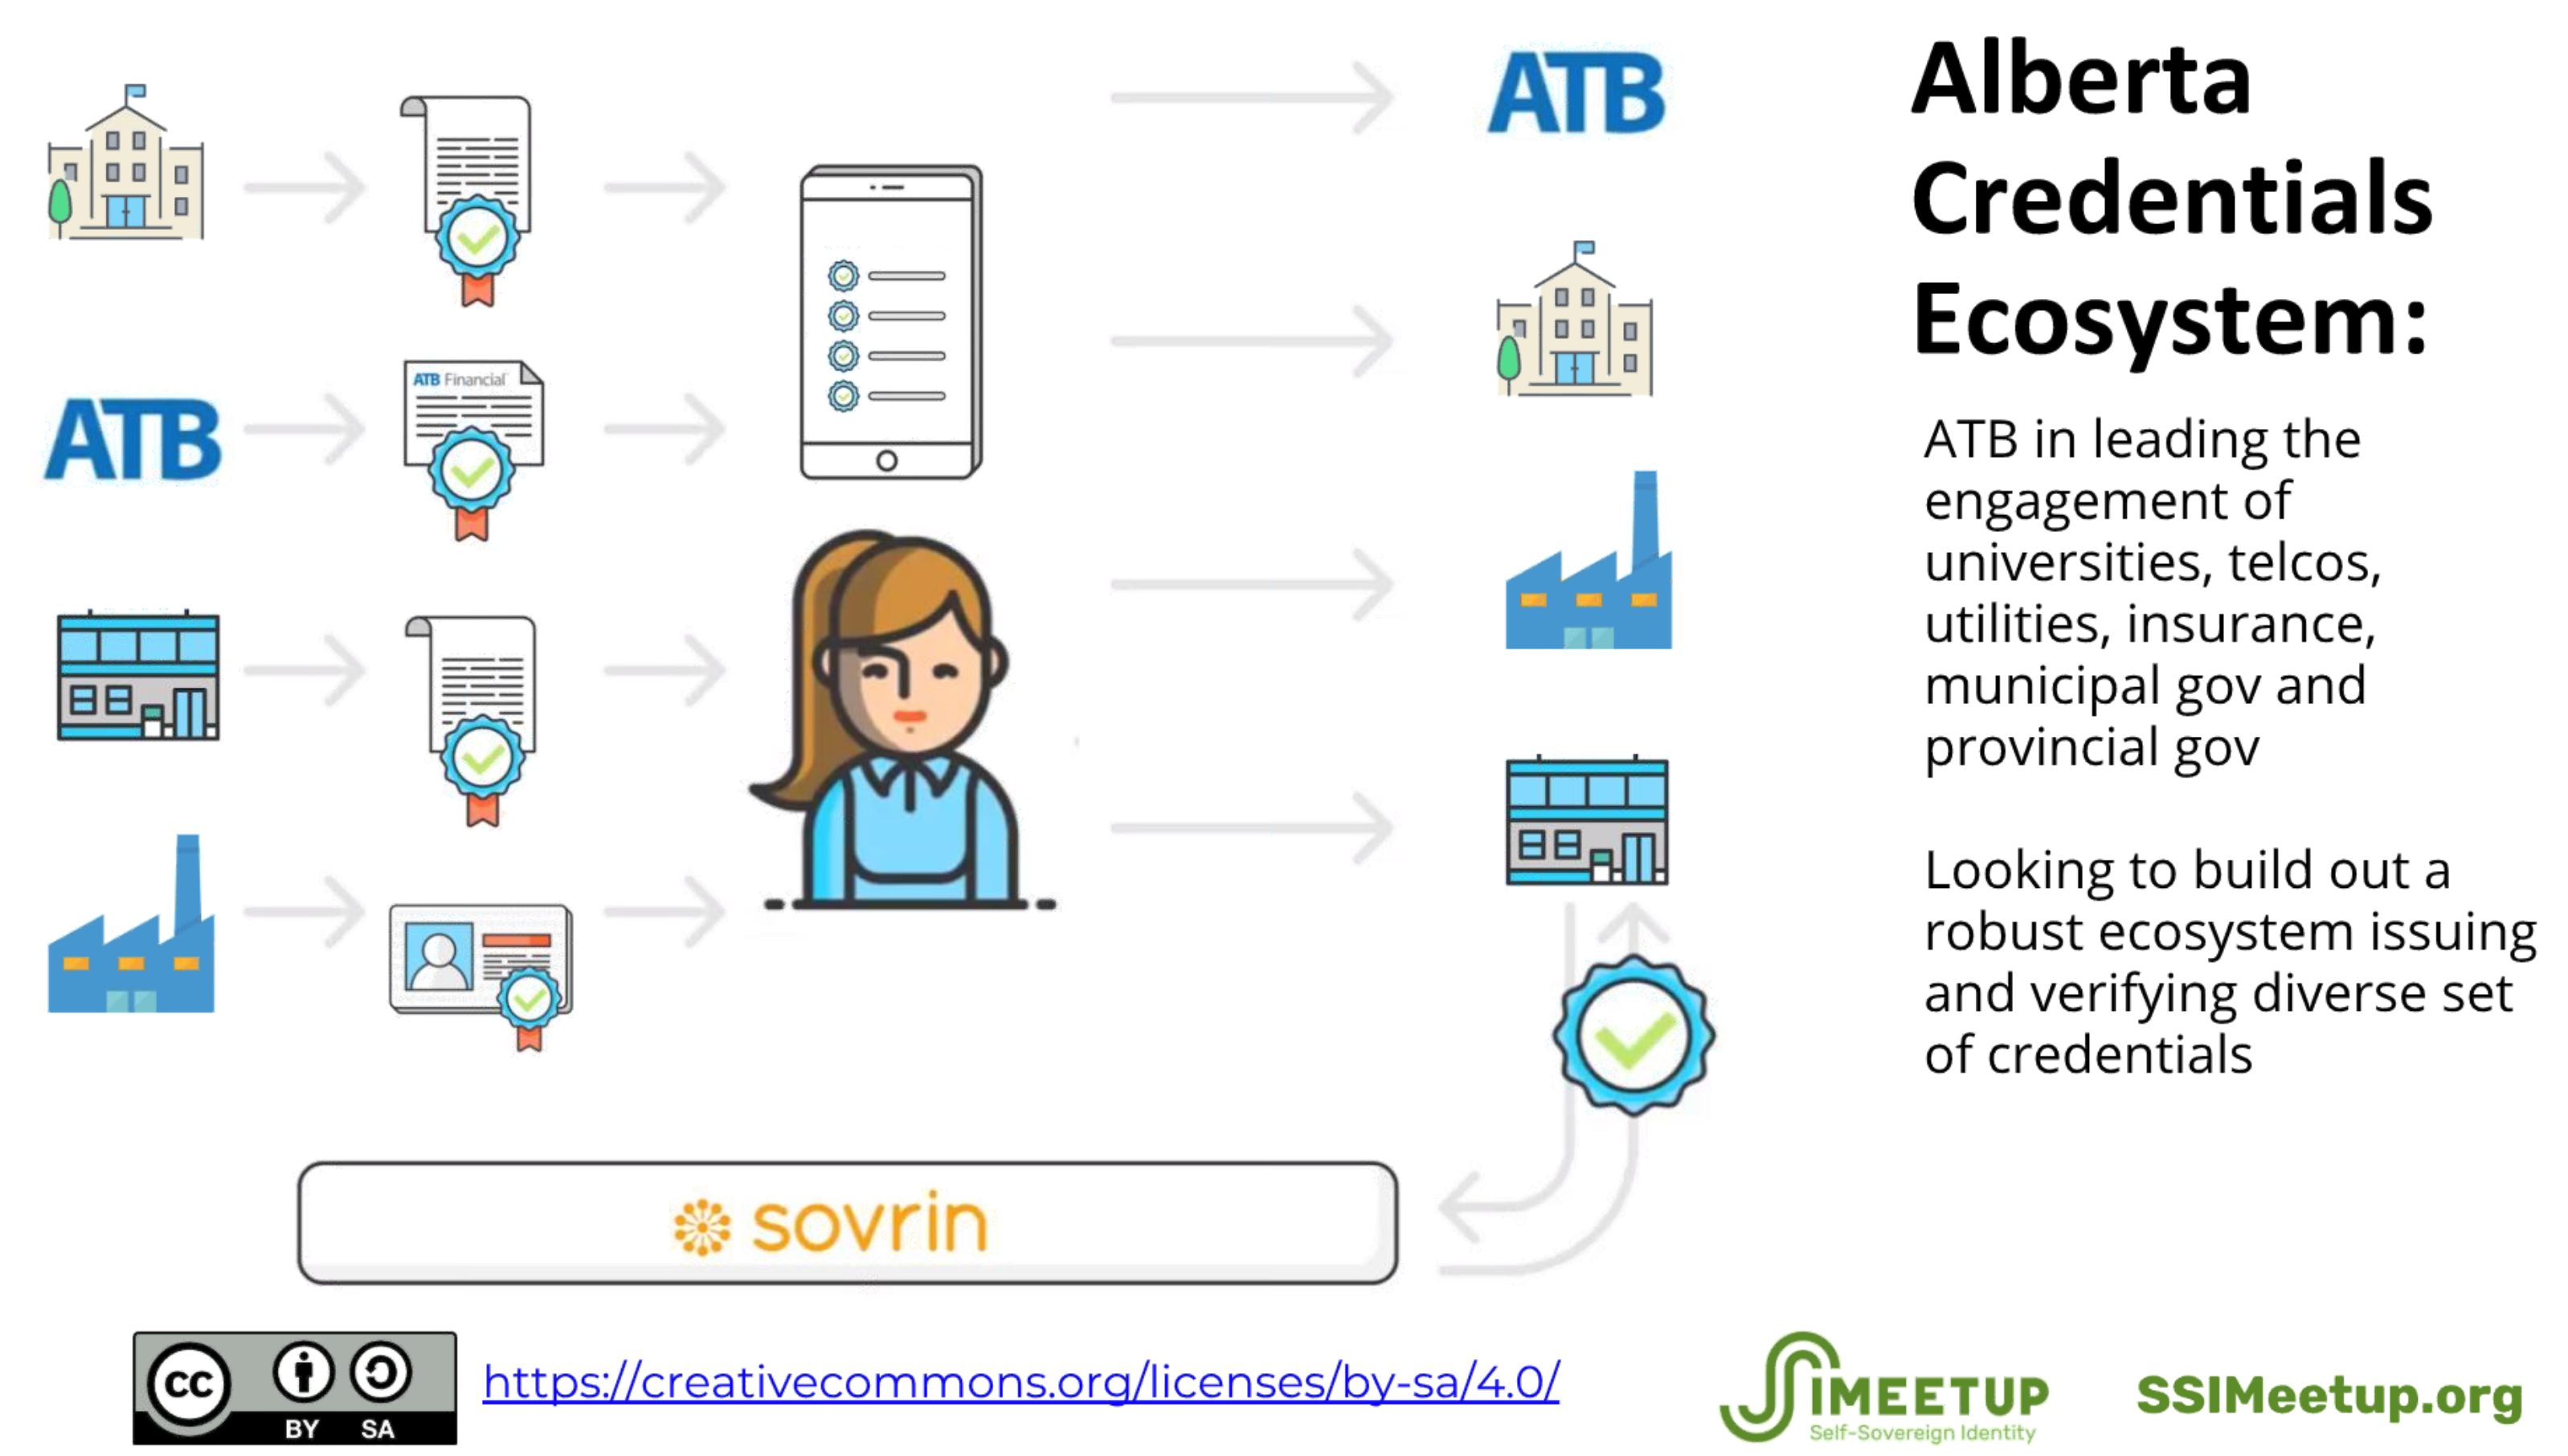
\includegraphics[height=6cm]{../pics/case_studies/alberta-credentials-ecosystem}
		\captionsetup{justification=centering}
		\caption{from \cite{ssimeetup201902:atb-slides}}
	\end{figure}
}

%\subsection{UK}
%\frame{
%	% counter example: cost 130 million pounds up to 2018, 7 years of work with not much -see https://www.computerweekly.com/blog/Computer-Weekly-Editors-Blog/Verify-on-the-verge-what-does-it-mean-for-GDS
%	\frametitle{GOV.UK Verify}
%	\framesubtitle{\url{https://www.gov.uk/government/publications/introducing-govuk-verify/introducing-govuk-verify}}
%	\begin{figure}
%		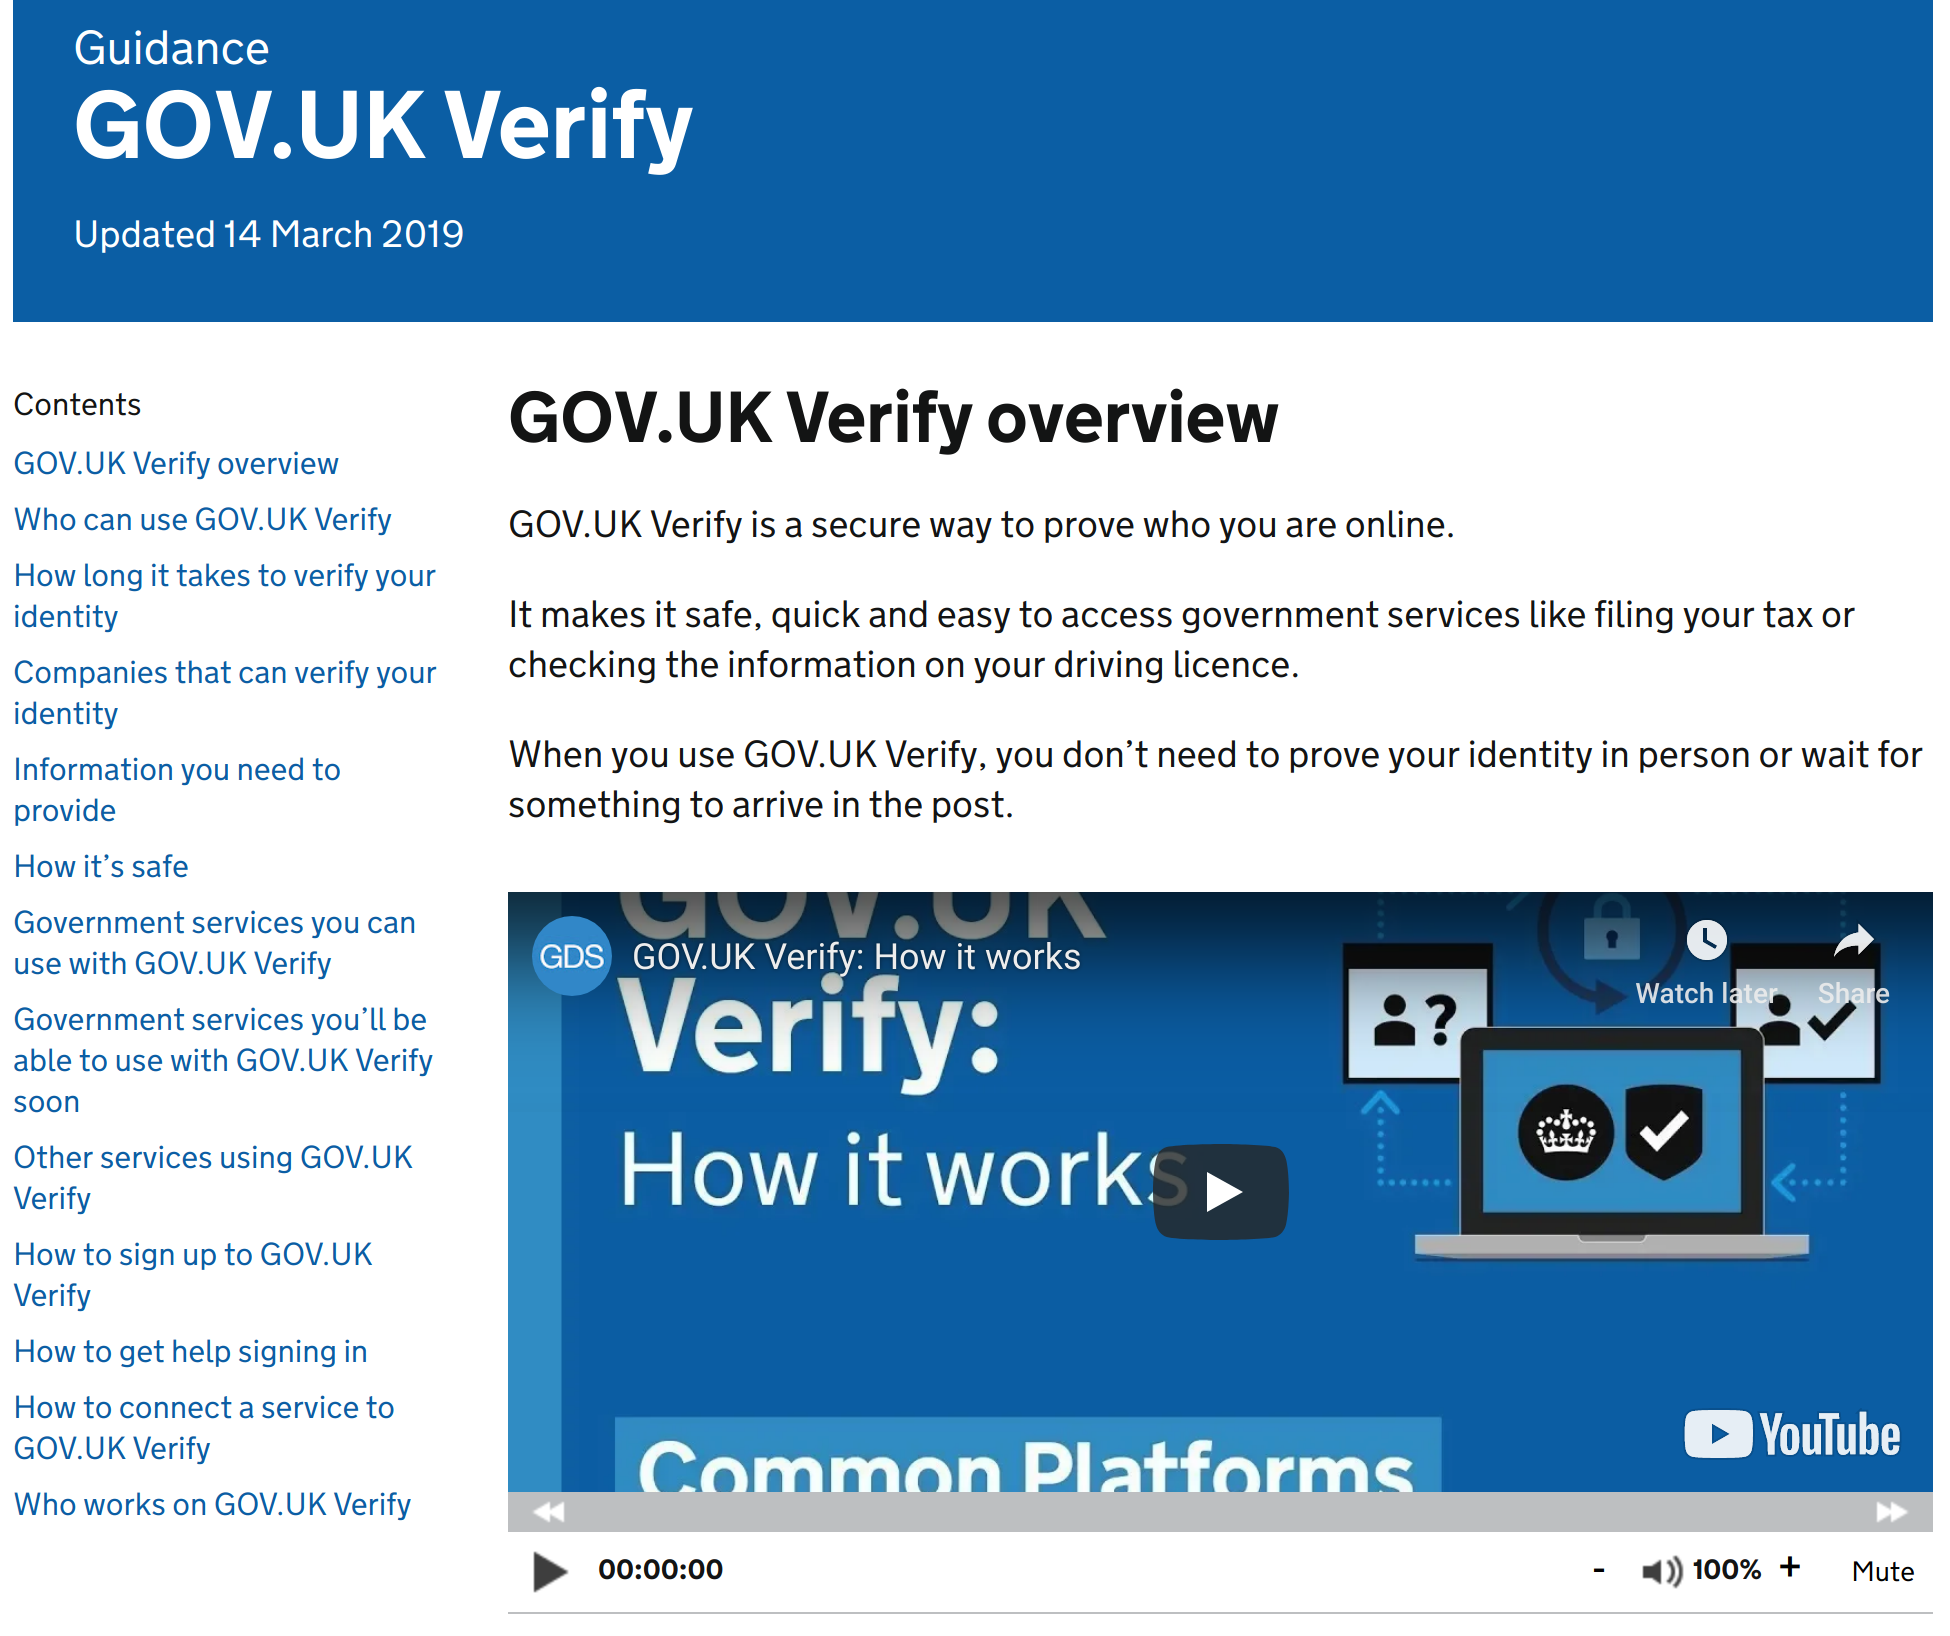
\includegraphics[height=6cm]{../pics/identity/gov-uk-verify}
%	\end{figure}
%}

%\frame{
%	\frametitle{The Open Identity Exchange}
%	\framesubtitle{\url{https://oixuk.org/}}
%	\begin{figure}
%		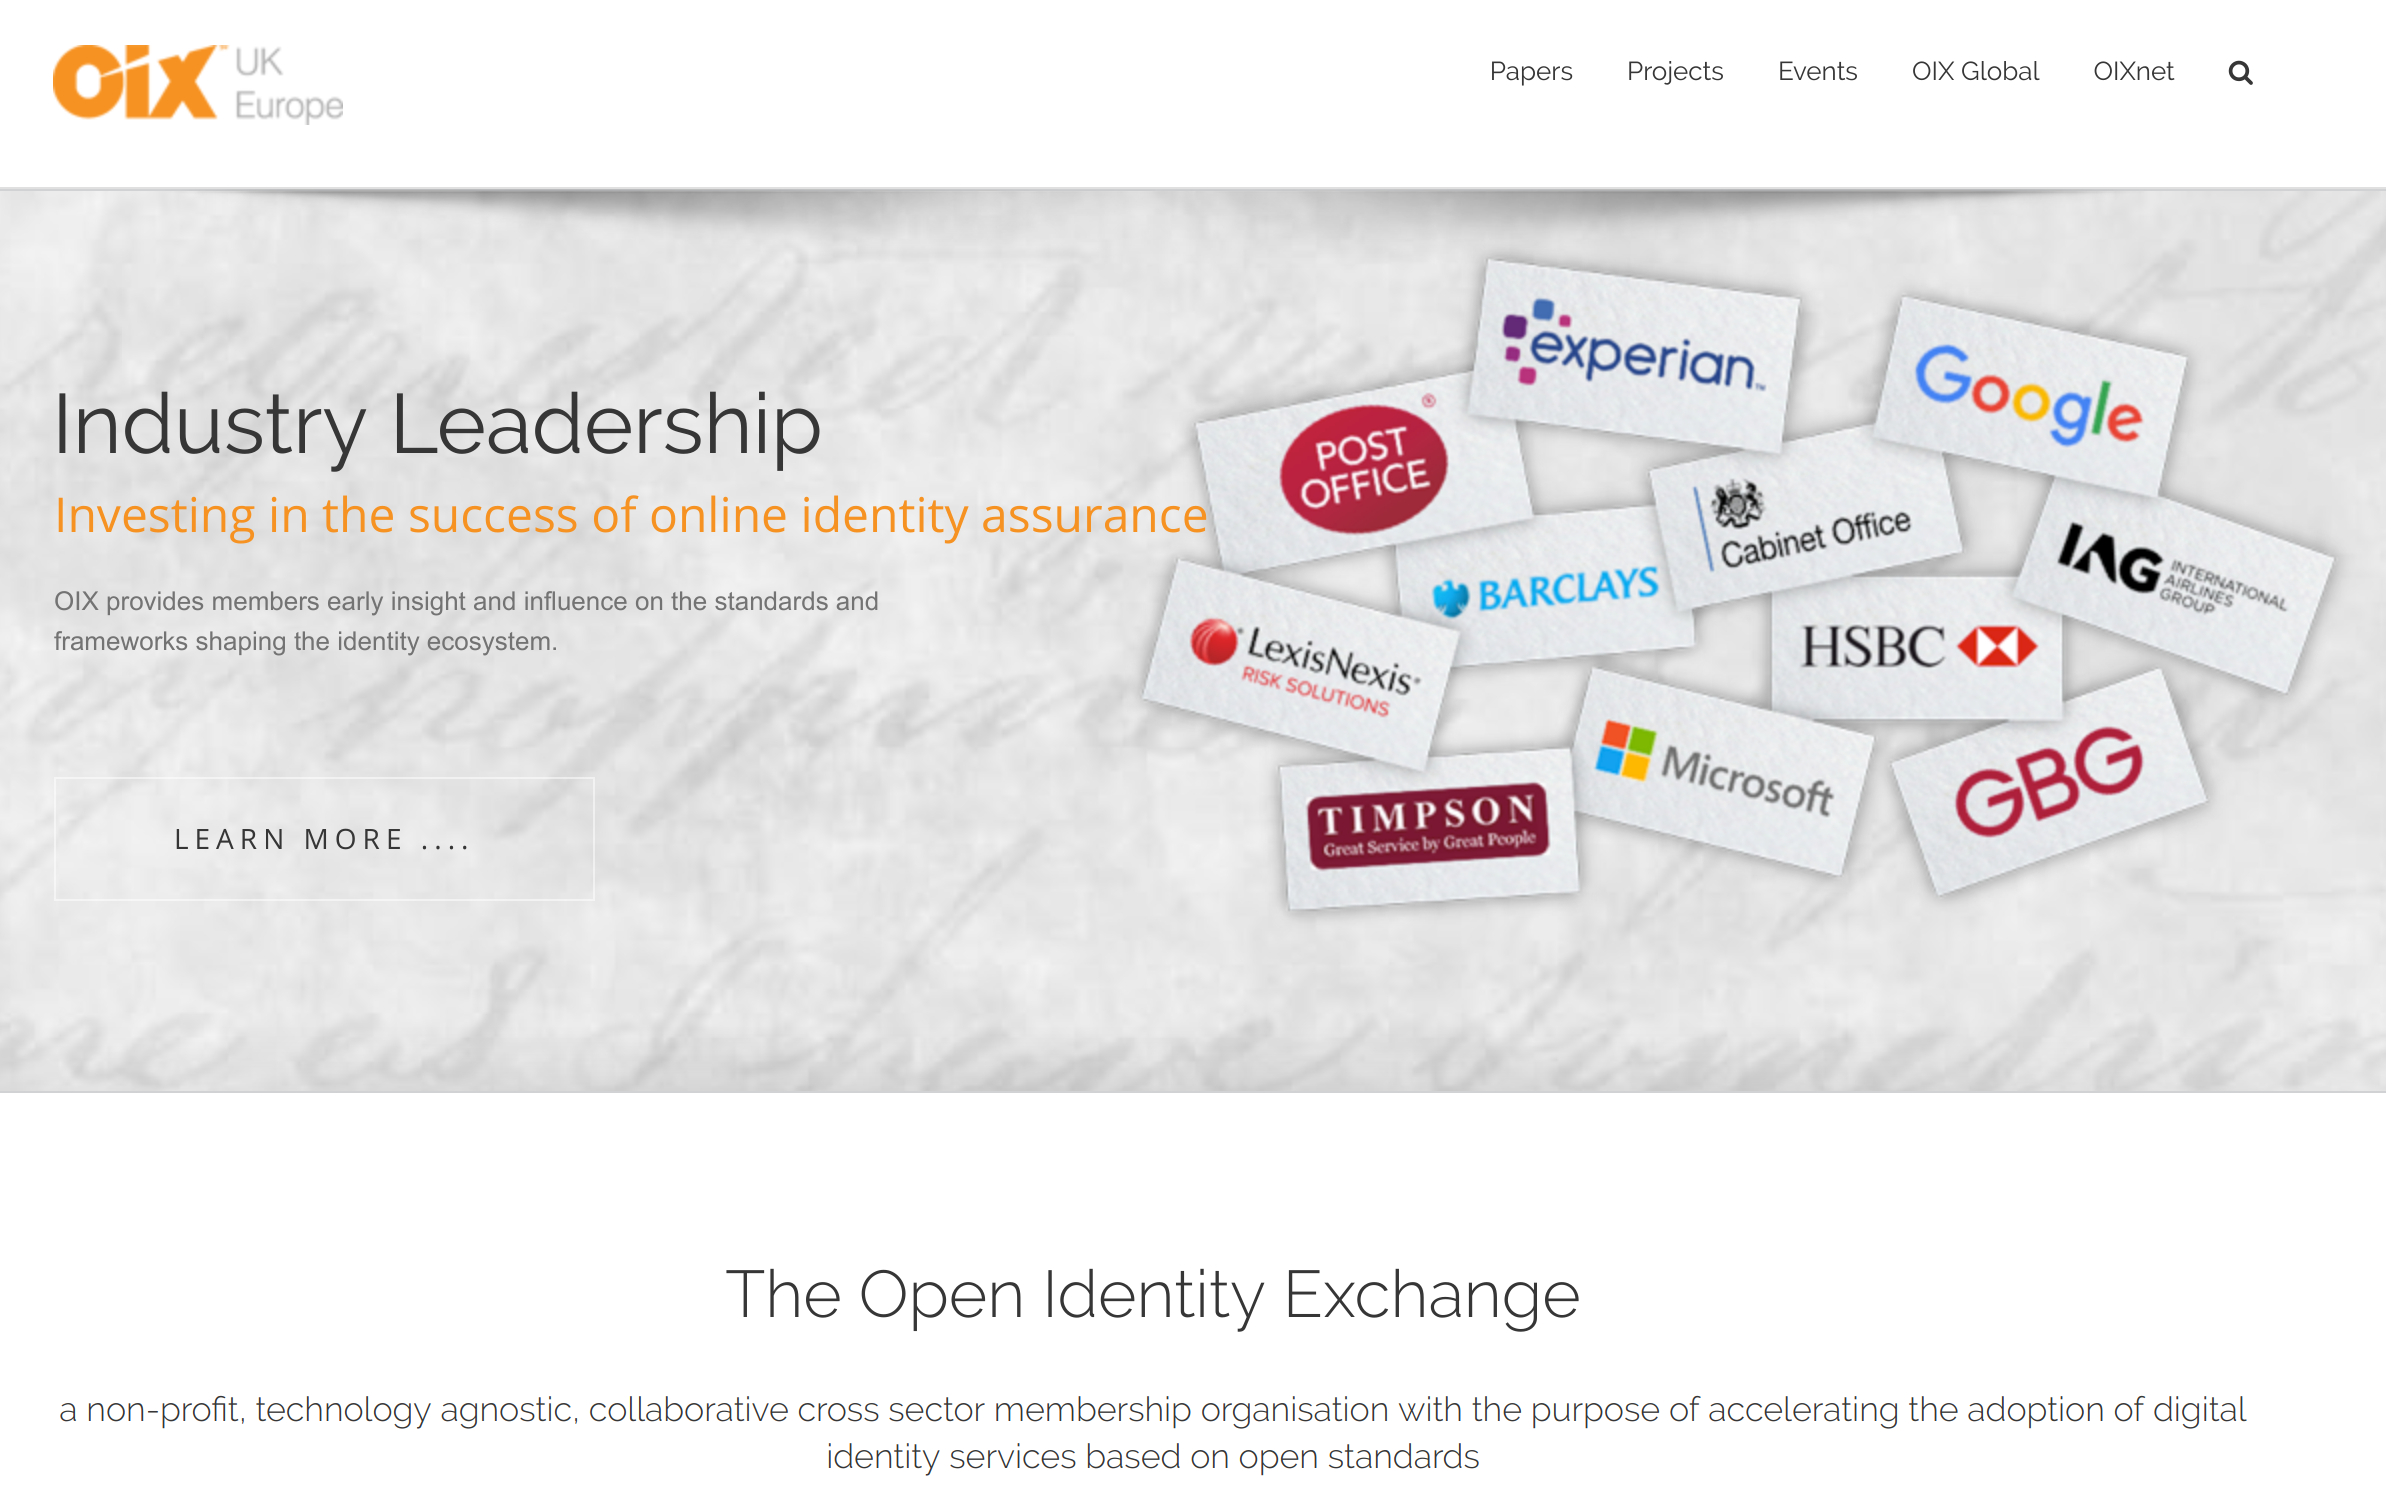
\includegraphics[height=6cm]{../pics/identity/oixuk-org}
%	\end{figure}
%}


\frame{
	\frametitle{Want to learn more about Blockchain?}
	\begin{figure}
		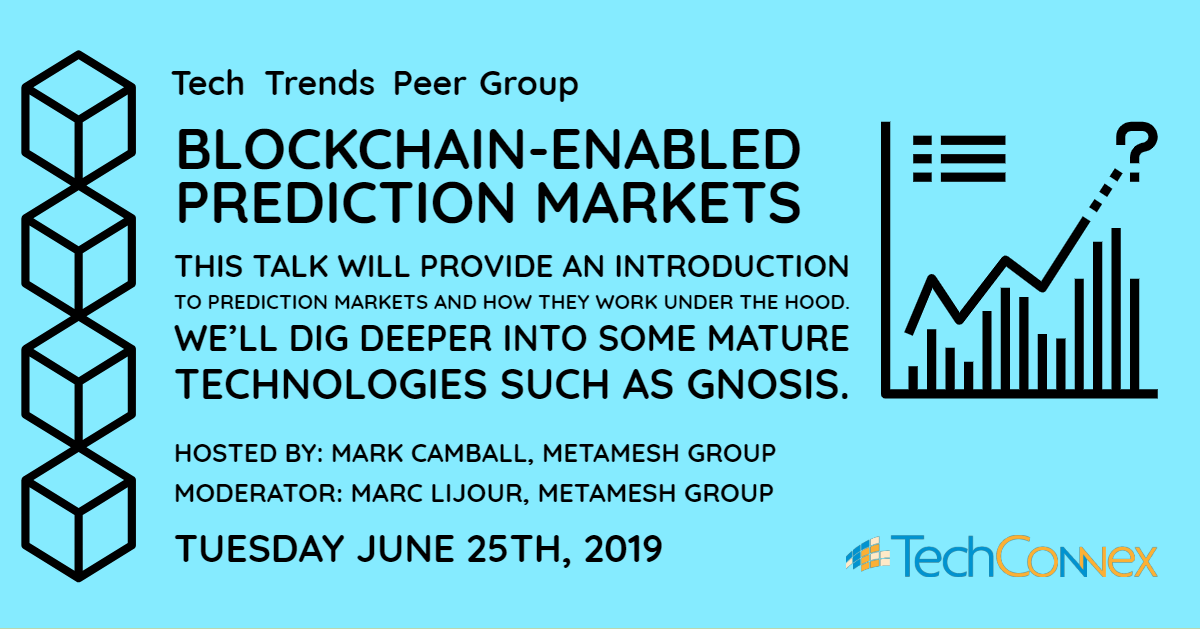
\includegraphics[height=6cm]{../pics/case_studies/techconnex-2019-06-25}
		\captionsetup{justification=centering}
	\end{figure}
}








